\documentclass[11pt,a4paper]{article}

\usepackage[T1]{fontenc}
\usepackage[utf8]{inputenc}
\usepackage[margin=1in]{geometry}
\usepackage{amsmath,amssymb}
\usepackage{graphicx}
\usepackage{booktabs}
\usepackage{array}
\usepackage{tabularx}
\usepackage{xcolor}
\usepackage{listings}
\usepackage{caption}
\usepackage{float}
\usepackage{subcaption}
\usepackage{enumitem}
\usepackage[parfill]{parskip}
\usepackage{titlesec}
\usepackage[expansion=false]{microtype}
\usepackage[hidelinks]{hyperref}
\emergencystretch=3em
\newcolumntype{Y}{>{\raggedright\arraybackslash}X}

% Float placement: fill pages with text, put float-only pages at the top
% (default LaTeX centres them vertically, which leaves large white gaps).
\renewcommand{\topfraction}{0.9}
\renewcommand{\bottomfraction}{0.8}
\renewcommand{\textfraction}{0.07}
\renewcommand{\floatpagefraction}{0.75}
\setcounter{topnumber}{3}
\setcounter{bottomnumber}{2}
\setcounter{totalnumber}{5}
\makeatletter
\setlength{\@fptop}{0pt}
\setlength{\@fpsep}{14pt}
\setlength{\@fpbot}{0pt plus 1fil}
\makeatother
\setlength{\textfloatsep}{12pt plus 2pt minus 4pt}
\setlength{\floatsep}{10pt plus 2pt minus 2pt}
\captionsetup{font=small,skip=4pt}

% Section style matching the group template: "1. Title"
\titleformat{\section}{\normalfont\Large\bfseries}{\thesection.}{0.5em}{}
\titleformat{\subsection}{\normalfont\large\bfseries}{\thesubsection}{0.8em}{}
\titleformat{\subsubsection}{\normalfont\normalsize\bfseries}{\thesubsubsection}{0.8em}{}

\definecolor{codebg}{HTML}{F6F5F2}
\definecolor{codekw}{HTML}{1C5CAB}
\definecolor{codecm}{HTML}{6B6A66}
\lstset{
  language=C++, basicstyle=\ttfamily\footnotesize, backgroundcolor=\color{codebg},
  keywordstyle=\color{codekw}\bfseries, commentstyle=\color{codecm}\itshape,
  frame=single, rulecolor=\color{codebg}, framesep=4pt, xleftmargin=6pt, xrightmargin=6pt,
  columns=fullflexible, keepspaces=true, breaklines=true, showstringspaces=false,
  morekeywords={atomic,memory_order_acquire,memory_order_release,memory_order_relaxed,memory_order_acq_rel,uint64_t,Cost,Key}
}

% Placeholder marker for parts the group still has to fill in
\newcommand{\todo}[1]{\textcolor{red!70!black}{\textbf{[TODO: #1]}}}

\newcommand{\Astar}{A\textsuperscript{*}}
\newcommand{\HDA}{HDA\textsuperscript{*}}
\newcommand{\NAMOA}{NAMOA\textsuperscript{*}}

\begin{document}

% Section: titlepage (\input from main.tex)
\begin{titlepage}
\centering
{\large VIETNAM NATIONAL UNIVERSITY -- HO CHI MINH CITY\par}
{\large\bfseries HO CHI MINH CITY UNIVERSITY OF TECHNOLOGY\par}
{\large FACULTY OF COMPUTER SCIENCE AND ENGINEERING\par}
\vspace{1cm}
\IfFileExists{figures/logo-hcmut.png}{%
  
\includegraphics[width=7cm]{figures/logo-hcmut.png}\par}{}
\vspace{1cm}
{\LARGE\bfseries Parallel Computing\par}
\vspace{0.4cm}
{\large A/Prof. Dr. Tran Van Hoai, Dr. Diep Thanh Dang\par}
\vspace{1.2cm}
{\Large\bfseries Assignment 2\par}
\vspace{0.4cm}
{\Large Sequential and Parallel A* Search\\ on the Ho Chi Minh City Road Network\par}
\vspace{1.2cm}
\begin{tabular}{lll}
\toprule
\textbf{Member} & \textbf{Student ID} & \textbf{Test platform} \\
\midrule
Pham Hoang Son & 2570315 & \todo{platform} \\
Nguyen Hoang Nam & 2570460 & \todo{platform} \\
Nguyen Dinh Khanh & 2570227 & Platforms A, B (Apple M5) \\
\bottomrule
\end{tabular}
\vfill
Source code: submitted with this report (\texttt{Assignment2\_ParallelAstar.zip})\\[0.3cm]
{\large November 4, 2026\par}
\end{titlepage}

\tableofcontents
\newpage

% Section: introduction (\input from main.tex)
\section*{Introduction}
\addcontentsline{toc}{section}{Introduction}

A* is the standard algorithm for finding a shortest path between two places in
a road network. It is a best-first search: it always expands the open node with
the smallest estimate $f = g + h$, where $g$ is the cost already paid and $h$ is
a heuristic estimate of the cost still to go. Making A* parallel is hard for
exactly that reason: the whole search is organised around one global
priority queue, and every thread wants the same minimum element. This report
documents our implementation and evaluation of A* and of the data structures
it needs, in C++17, following the four parts of Assignment~2:

\begin{enumerate}[nosep]
  \item \textbf{Sequential A*} on the real road network of urban Ho Chi Minh
        City (203\,396 nodes), extended to a \emph{dynamic and uncertain}
        heuristic, to the lecturer's time-dependent speed model, and to a
        \emph{vector-valued} $f$ (multi-objective A*, \NAMOA). We also checked
        the A* pseudocode of the lecture and the reference notebook
        \texttt{osm-astar.ipynb}.
  \item \textbf{A concurrent set as a sorted linked list} --- all four
        synchronization strategies (coarse-grained, fine-grained,
        optimistic, lazy), each with \texttt{std::mutex}, a TTAS spinlock
        and a TTAS lock with exponential backoff.
  \item \textbf{Parallel A*} --- the sequential algorithm and the sorted list
        adapted so that they can be merged, compared with a locked binary heap
        and with Hash-Distributed A* (\HDA).
  \item \textbf{Other optimizations (optional)} --- ALT landmarks, incumbent
        pruning, heuristic memoisation and a synchronisation window for \HDA.
\end{enumerate}

For every part we describe the algorithm and its memory-ordering choices, the
test used to establish correctness, and a performance and scalability study on
three shared-memory platforms. Section~\ref{sec:setup} describes the data and
the shared methodology; Sections~\ref{sec:seq}--\ref{sec:opt} cover the four
parts; Section~\ref{sec:cross} compares platforms and Section~\ref{sec:threats}
discusses limitations.

% Section: setup (\input from main.tex)
\section{Experimental Setup and Methodology}
\label{sec:setup}

\subsection{Code organization}

The project is a single \texttt{Makefile} build (C++17, \texttt{-O2},
\texttt{-pthread}) with header-only implementations, separate correctness
tests, and benchmark drivers:

\begin{center}
\small
\begin{tabularx}{\linewidth}{>{\ttfamily}l X}
\toprule
\textrm{\textbf{File}} & \textbf{Content} \\
\midrule
src/graph.hpp      & CSR road graph with integer costs, admissible straight-line bound, CSV loader \\
src/seq\_astar.hpp & Part 1: Dijkstra (test oracle), generic A*, Euclidean / uncertain / dynamic / ALT / costly heuristics, \NAMOA \\
src/clist.hpp      & Part 2: \texttt{CoarseList}, \texttt{FineList}, \texttt{OptimisticList}, \texttt{LazyList}; \texttt{MutexLock}, \texttt{TTASLock}, \texttt{BackoffLock}; \texttt{removeMin} \\
src/par\_astar.hpp & Part 3: parallel A* over a shared open list (any list, or a locked heap); \HDA{} with optional $f$-window \\
src/route.cpp      & command-line route planner (GeoJSON output) \\
tests/             & \texttt{test\_seq}, \texttt{test\_clist}, \texttt{test\_par} (also built with ThreadSanitizer) \\
bench/             & \texttt{bench\_seq}, \texttt{bench\_clist}, \texttt{bench\_astar} \\
scripts/           & \texttt{build\_graph.py} (OSM $\rightarrow$ graph), figure and table scripts \\
run\_all.sh, run\_mac.sh & build, run all tests, then the full benchmark sweep on one platform \\
\bottomrule
\end{tabularx}
\end{center}

All benchmarks write CSV files named \texttt{results/<experiment>\_<platform>.csv};
all tables and figures in this report are regenerated from those files.

\subsection{Road network}

The lecturer's notebook downloads the drive network of the whole city with
OSMnx. From our networks the OSMnx services were not usable: Nominatim, which
turns the place name into a boundary, was blocked, and all public Overpass
servers were overloaded (HTTP 429, 502, 504). We therefore built the graph
from Geofabrik's OpenStreetMap extract of Vietnam (\texttt{vietnam-latest.osm.pbf},
332\,MB, \copyright{} OpenStreetMap contributors, ODbL) with
\texttt{scripts/pbf\_to\_graph.py}:

\begin{itemize}[nosep]
  \item The bounding box covers urban Ho Chi Minh City (latitude 10.65--10.92,
        longitude 106.55--106.88): Districts 1--12, Binh Thanh, Phu Nhuan, Go
        Vap, Tan Binh, Tan Phu, Binh Tan, Thu Duc City, Nha Be and the urban
        parts of Binh Chanh and Hoc Mon. It contains both end points of the
        lecturer's example.
  \item It keeps every road a motorbike may use (motorway to residential
        roads, links, living streets and service roads except parking aisles
        and driveways; \texttt{access=no/private} removed) and honours one-way
        tags and roundabouts.
  \item Like OSMnx, it simplifies the graph: nodes are kept only where roads
        end, meet, or leave the box, and an edge gets the summed length of the
        road segments it replaces.
  \item It keeps the largest strongly connected component, so every pair of
        nodes has a route.
\end{itemize}

The result has \textbf{203\,396 nodes and 455\,837 directed edges}
(Figure~\ref{fig:map}). The lecturer's example, from Thu Thiem
(10.768856, 106.725019) to Thu Duc (10.839613, 106.845798), is a 19.1\,km
route that A* with ALT finds after 5\,058 expansions, against 154\,943 for
Dijkstra. Part~2 does not use the graph. During development we also used a
small extract of the city centre (33\,718 nodes); \texttt{osm-astar-fixed.ipynb}
can still run on it.

Every edge carries three integer costs: \emph{length} in millimetres,
free-flow \emph{time} in milliseconds (from \texttt{maxspeed}, or a per-class
default of 10--60\,km/h), and rush-hour \emph{congested time} (free-flow time
multiplied by 1.0--2.6 depending on the road class, because main roads are the
most congested). We use integers on purpose: sequential and parallel results
can then be compared for exact equality, with no floating-point tolerance.
The time-dependent model of Section~\ref{sec:seq-td} uses the lecturer's speed
profile instead.

\begin{figure}[H]
\centering
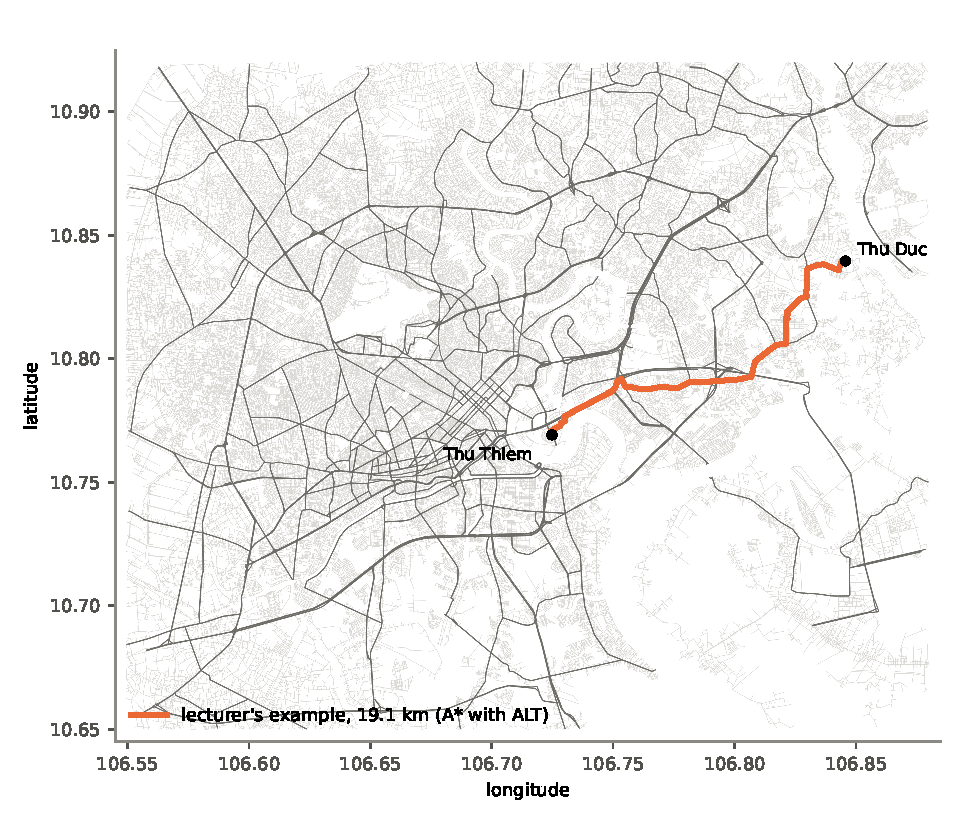
\includegraphics[width=0.8\linewidth]{figures/fig1_map.pdf}
\caption{The road graph of urban Ho Chi Minh City (major roads darker) and the
lecturer's example query. Every algorithm in this report returns this route
(\texttt{./bin/route 10.768856 106.725019 10.839613 106.845798 --algo alt --data data\_city}).}
\label{fig:map}
\end{figure}

\subsection{Parameters and measurement}

\begin{center}
\small
\begin{tabularx}{\linewidth}{l Y Y}
\toprule
\textbf{Part} & \textbf{Swept parameters} & \textbf{Fixed amount of work} \\
\midrule
1 Sequential A* & heuristic, metric (length, time), error $\varepsilon\in\{0.1,0.3,0.5,1,2\}$, departure time & 200 random queries with straight-line distance $>1$\,km; 40 bi-objective queries (0.5--4.5\,km); 40 simulated trips ($\ge 3.5$\,km) \\
2 Lists  & list $\times$ lock (12 variants), threads $\in\{1,2,4,8,16\}$, workload mix & key range 1\,000, half pre-filled; each run lasts 0.4\,s \\
3 Parallel A* & version (12 parallel + sequential), heuristic (4), threads $\in\{1,2,4,8,16\}$ & 20 long queries ($>5$\,km, about 99\,000 Dijkstra expansions each) \\
\bottomrule
\end{tabularx}
\end{center}

Part~1 reports the mean time per query. Part~2 reports throughput in million
operations per second; Part~3 reports the wall time to answer all 20 queries
one after another, so thread creation and joining is included once per query.
Each Part~2 and Part~3 configuration is repeated 3 times and we report the
\textbf{median}. Time is measured with \texttt{std::chrono::steady\_clock}.
Part~2 used threads $\in\{1,2,4,8,16\}$ on Platform~A, $\{1,2,4,8\}$ on
Platforms~B and~C, and $\{1,2,4,8,10,16,20,32\}$ on Platform~D; Part~3 used up to twice the hardware threads (capped at 32 on D):
$\{1,\dots,16\}$ on A, $\{1,2,4,8\}$ on B, $\{1,2,4\}$ on C, and $\{1,2,4,8,10,16,20,32\}$ on D. Shaded regions in the figures mark thread counts that exceed
the hardware threads available. An extended sweep (\texttt{run\_ext.sh}) on Platform~D additionally measures 5--7 repetition spread, persistent \texttt{ThreadPool} vs.\ per-query spawning, physical-core-first pinning, key ranges up to 50\,000, \texttt{TTASLock} in Part~3, the \texttt{TIME} metric, and \HDA{} $f$-window tuning.

Solution \emph{quality} is measured as cost divided by the exact optimum from
Dijkstra. All exact algorithms (every parallel version included) reach a ratio
of exactly 1.000000 in every run, so quality only differs in the deliberately
inexact variants of Sections~\ref{sec:seq-dyn} and~\ref{sec:seq-td}.

\subsection{Platforms}

The assignment requires at least as many platforms as group members.
Table~\ref{tab:platforms} lists them.

\begin{table}[H]
\centering
\scriptsize
\caption{Shared-memory platforms used in the study.}
\label{tab:platforms}
\begin{tabularx}{\linewidth}{l YYYY}
\toprule
 & \textbf{Platform A} & \textbf{Platform B} & \textbf{Platform C} & \textbf{Platform D} \\
\midrule
Machine       & MacBook Pro (Apple M5), native & Linux VM on the same MacBook Pro & Cloud virtual machine & Workstation (bare-metal) \\
CPU           & Apple M5, 4P + 6E cores & Apple M5 (4 vCPUs) & Intel Xeon @ 2.10\,GHz & Intel Xeon W-2255 @ 3.70\,GHz \\
Cores / HW threads & 10 / 10 & 4 / 4 & 2 / 2 & 10 / 20 (SMT) \\
Memory        & 16\,GiB & 4\,GiB & 8\,GiB & 61\,GiB \\
OS            & macOS 27.2 & Ubuntu 22.04 (aarch64) & Ubuntu 24.04 (x86-64) & Ubuntu (x86-64, Linux 7.0) \\
Compiler / C++ library & Apple Clang 21.0, libc++ & GCC 11.4, libstdc++ & GCC 13.3, libstdc++ & GCC 15.2, libstdc++ \\
Memory model  & ARMv8 (weak) & ARMv8 (weak) & x86-64 TSO & x86-64 TSO \\
\bottomrule
\end{tabularx}
\end{table}

The platforms differ in instruction set and memory model, operating system and
scheduler, C++ library, and core count. Two of them are ARM machines, so the
acquire/release orderings of our lock-free list traversals are exercised on a
weak memory model and not only on x86. Platform~A is heterogeneous (only
4 of its 10 cores are performance cores), whereas Platform~D provides 10 uniform
physical cores (20 hardware threads with SMT) without hypervisor scheduling.
One caveat applies to Platform~A: random query pairs are drawn with
\texttt{std::\allowbreak uniform\_int\_\allowbreak distribution}, whose algorithm differs between libc++
and libstdc++. Platform~A therefore answers a different (statistically
equivalent) query set from B, C, and D (which share identical libstdc++ queries). Speed-ups are always computed against the
sequential run on the same platform and the same queries, so they remain
comparable.

% Section: sequential (\input from main.tex)
\section{A* in the Sequential World}
\label{sec:seq}

\subsection{Implementation}

\texttt{astar()} is the textbook algorithm. OPEN is a binary heap of
$(f, v)$ pairs with lazy deletion: instead of decreasing a key, a node is
pushed again and outdated entries are skipped when popped. $g$-values and
parent pointers are arrays indexed by node. The function is a template over
the heuristic and the edge-weight functor, so the same code serves every
variant in this section, including the dynamic ones:

\begin{lstlisting}
while (!open.empty()) {
  auto [f, u] = open.top(); open.pop();
  if (closed[u]) continue;                                   // duplicate entry
  if (H::dynamic) {                                          // h may have changed
    Cost fnow = g[u] + h(u);
    if (fnow > f && !open.empty() && fnow > open.top().first) {
      open.push({fnow, u}); continue;                        // lazy re-keying
    }
  } else if (f > g[u] + h(u)) continue;                      // outdated entry
  closed[u] = 1; h.tick();
  if (u == t) break;
  for (auto e = G.begin(u); e != G.end(u); ++e) {
    Cost ng = g[u] + W(*e);
    if (ng < g[e->to]) {
      if (closed[e->to]) closed[e->to] = 0;                  // re-open
      g[e->to] = ng; parent[e->to] = u; open.push({ng + h(e->to), e->to});
    }
  }
}
\end{lstlisting}

\paragraph{Heuristic.} The default $h$ is the great-circle (haversine) distance
to the target. For the time metric it is divided by $v_{\max}$, the highest
speed that occurs anywhere in the graph. Edge costs are rounded \emph{up} to
whole millimetres or milliseconds and $h$ is rounded \emph{down}, so $h$ is
admissible and consistent by construction; Section~\ref{sec:seq-test} checks
this on every edge. A consistent $h$ never re-opens a closed node, so the
re-opening branch above is needed only for the heuristics of
Section~\ref{sec:seq-dyn}.

% Subsection: review of the lecture material (\input from sections/sequential.tex)
\subsection{Checking the lecture's pseudocode and reference notebook}
\label{sec:review}

The lecture slides ask to ``check the correctness of the left algorithm'' (the
A* pseudocode on slides 9--10), and the reference notebook
\texttt{osm-astar.ipynb} is marked ``not yet verified''. We checked both.

\paragraph{Pseudocode (slides 9--10).}
\begin{itemize}[nosep]
  \item The selected vertex $u$ is added to $C$ but \textbf{never removed from
        $O$}. The next iteration selects the same $u$ again, so the loop never
        progresses. The fix is $O := O \setminus \{u\}$ after the selection.
  \item Neighbours already in $C$ are skipped. This is correct only for a
        \emph{consistent} $h$. With a dynamic or uncertain $h$ (the question on
        slide~10) a closed vertex can later be reached with a smaller
        $g$, and it must be re-opened (Section~\ref{sec:seq-dyn}).
  \item When $O$ becomes empty without reaching $d$, the procedure ends
        without reporting that no path exists.
\end{itemize}

\paragraph{Reference notebook.} We ran the notebook's
\texttt{astar\_shortest\_path} unchanged on our graph, loaded as an OSMnx-style
\texttt{MultiDiGraph}, and compared it with \texttt{networkx} shortest paths.
Table~\ref{tab:review} lists what we found. The most serious problem is B9: in
an OSMnx \texttt{MultiDiGraph}, \texttt{graph[u]} maps each neighbour to a
dictionary of \emph{parallel edges} (\texttt{\{0: \{'length': ...\}\}}), so
\texttt{edge\_data.get('length', 1)} always returns the default 1. Every road
segment then costs 1\,m, and the code minimises the number of segments. This
explains the weight printed in the notebook: 0.34\,min for a trip across the
city. On our graph the same example is a 19.1\,km route that takes 41\,min with
the lecturer's speed profile.

\begin{table}[H]
\centering
\small
\caption{Problems found in \texttt{astar\_shortest\_path} of the reference
notebook, measured with the code unchanged on 60 random queries on our city
graph.}
\label{tab:review}
\begin{tabularx}{\linewidth}{l >{\raggedright\arraybackslash}p{4.6cm} Y}
\toprule
 & \textbf{Problem} & \textbf{Effect and fix} \\
\midrule
B1 & \texttt{f\_score\_neighbor = g\_score + h\_score} uses the \emph{current} node's $g$ and $h$ & the queue is not ordered by the neighbour's $f$, so the search is not A*. Fix: $g_{\mathrm{nb}} + h_{\mathrm{nb}}$ \\
B2 & \texttt{t = t + ...} inside the neighbour loop & the current node's clock grows with every neighbour scanned. Fix: a separate $t_{\mathrm{nb}}$ \\
B3 & \texttt{speeds[floor(t)]}, $t$ in minutes, 20 slots & \texttt{IndexError} for trips longer than 20\,min; hidden only by B9 (with B9 fixed, the code crashes). Fix: cyclic profile \\
B4 & Euclidean distance on longitude/latitude \emph{degrees} & $h \approx 10^{-4}$\,min: the search expands as many nodes as Dijkstra (198\,718 against 198\,722 on a long query). Fix: great-circle distance in metres \\
B5 & $h = d / \textit{speed}(t)$ & over-estimates when later slots are faster, so $h$ is not admissible (Section~\ref{sec:seq-td}). Fix: $d / v_{\max}$ \\
B6 & \texttt{shortest\_path\_at\_time} runs a full Dijkstra in every call of $h$ & 0.6\,s per generated node on the city graph; not admissible either (B5). Fix: one reverse Dijkstra per destination \\
B7 & edge time uses only the speed at departure & not FIFO: 6.3\% of random (departure, length) pairs arrive earlier when leaving later, so label-setting A* is not exact. Fix: integrate the speed over the slots \\
B8 & the whole path is copied into every queue entry; no best-$g$ check & $O(\text{path length})$ memory per entry and many useless duplicates. Fix: parent array \\
B9 & \texttt{edge\_data.get('length', 1)} on a \texttt{MultiDiGraph} & always 1: routes are 26\% longer than the shortest route on average (up to $2.2\times$), and the reported weight is 0.48\,min instead of 37.8\,min. Fix: minimum over parallel edges \\
B10 & returns \texttt{f\_score} as the path weight & wrong whenever B1 applies. Fix: return the arrival time minus the departure time \\
\bottomrule
\end{tabularx}
\end{table}

The corrected notebook (\texttt{notebooks/osm-astar-fixed.ipynb}) keeps the
original function next to the fixed one. On 60 random queries with four
departure times, the fixed time-dependent A* returns exactly the travel time
of an independent oracle and of the uninformed search
(Section~\ref{sec:seq-td}). Our C++ implementation follows the same
corrections.


\subsection{Dynamic and uncertain heuristic}
\label{sec:seq-dyn}

In a live navigation system the remaining cost comes from a predictor that is
noisy and changes while the search runs. We model both effects:

\begin{itemize}[nosep]
  \item \textbf{Uncertain $h$:} $h(v) = h_0(v)\,(1 + \varepsilon U)$ with
        $U \sim \mathcal{U}(-1, 1)$ drawn \emph{at every evaluation}. Two
        evaluations of the same node can return different values, like a
        noisy sensor.
  \item \textbf{Dynamic $h$:} $h_k(v) = h_0(v)\,\lambda(k)$ with
        $\lambda(k) = 1 + \varepsilon \sin(2\pi k/300)$, where $k$ is the
        number of expansions so far. This is a traffic forecast that is
        refreshed periodically during the search.
\end{itemize}

Both heuristics break the assumptions of textbook A* in three ways, and the
code handles each of them:

\begin{enumerate}[nosep]
  \item $h$ is no longer consistent and can over-estimate by up to a factor
        $1+\varepsilon$. A node can then be reached later with a smaller $g$,
        so closed nodes must be \textbf{re-opened}.
  \item The key stored in OPEN becomes \textbf{stale} when $h$ changes. On
        every pop the key is recomputed with the current $h$. If it is now
        larger than the next key in the heap, the node is pushed back instead
        of being expanded (lazy re-keying).
  \item The returned cost is recomputed along the final parent chain, because
        a re-opened ancestor may have improved after the goal was reached.
\end{enumerate}

Since $h \le (1+\varepsilon)\,h^*$ for every evaluation, the usual
weighted-A* argument bounds the result: $C^* \le C \le (1+\varepsilon)\,C^*$.

% Subsection: time-dependent travel times (\input from sections/sequential.tex)
\subsection{Time-dependent travel times (the lecturer's model)}
\label{sec:seq-td}

The reference notebook makes $h$ dynamic in a concrete way: the speed changes
with the time of day. A profile of 20 slots gives one network-wide speed per
slot (350--600\,m/min), and a trip that departs at time $t$ drives at
$\mathit{speeds}[\lfloor t \rfloor]$. Both the travel time of an edge and the
heuristic then depend on the time at which a node is reached. We implemented
this model in C++ (\texttt{td\_astar}, \texttt{SpeedProfile}) with three
corrections to the notebook (Section~\ref{sec:review}):

\begin{enumerate}[nosep]
  \item \textbf{FIFO edge times.} The time to drive an edge integrates the
        speed over every slot the edge spans. Leaving later can then never
        mean arriving earlier, which is the condition under which
        label-setting A* (and Dijkstra) remain exact for time-dependent costs.
        Using only the speed at departure, as the notebook does, violates this
        for 6.3\% of random (departure time, length) pairs.
  \item \textbf{Admissible heuristic.} $h(v) = d_{\mathrm{gc}}(v,t)/v_{\max}$,
        where $d_{\mathrm{gc}}$ is the great-circle distance and $v_{\max}$ the
        highest speed of the profile, never over-estimates, whatever the time.
        The notebook divides by the speed at the current time, which
        over-estimates whenever faster slots follow.
  \item \textbf{Cyclic profile,} so that trips longer than 20 slots stay
        inside the array.
\end{enumerate}

\paragraph{Testing.} Test T6 checks FIFO on 200\,000 random pairs, and runs
100 random queries at random departure times. Because the speed is the same on
every road at a given moment and travel is FIFO, the fastest route is the
shortest-length route, and its travel time is $\mathrm{arrive}(t_0, L^*) - t_0$.
This gives an oracle that does not share code with A*. Time-dependent A* and
time-dependent Dijkstra must both match it to $10^{-6}$\,min; they do on all
five platforms.

\begin{table}[H]
\centering
\small
\caption{Part 1: time-dependent A* with the lecturer's speed profile; 200
queries $\times$ 4 departure times. Expanded, re-opened and quality
(cost/optimum) are from Platform~C; B and C use the same queries. The road
distance $d_{\mathrm{road}}$ needs one reverse Dijkstra per destination, which
is not included in the time.}
\label{tab:td}
\begin{tabular}{l rrrrr r}
\toprule
Heuristic & ms (A) & ms (C) & expanded & re-opened & mean & worst \\
\midrule
$h = 0$ (time-dependent Dijkstra) & 6.6 & 19.8 & 104{,}414 & 0 & 1.000 & 1.000 \\
$h = d_{\mathrm{gc}} / v_{\max}$ & 4.3 & 12.8 & 44{,}367 & 0 & 1.000 & 1.000 \\
$h = d_{\mathrm{road}} / v_{\max}$ (one reverse Dijkstra) & 2.0 & 5.7 & 25{,}439 & 0 & 1.000 & 1.000 \\
$h = d_{\mathrm{gc}} / \mathit{speed}(t)$ (lecturer) & 4.5 & 16.2 & 62{,}804 & 45{,}665 & 1.045 & 1.288 \\
\bottomrule
\end{tabular}

\end{table}

\begin{figure}[H]
\centering
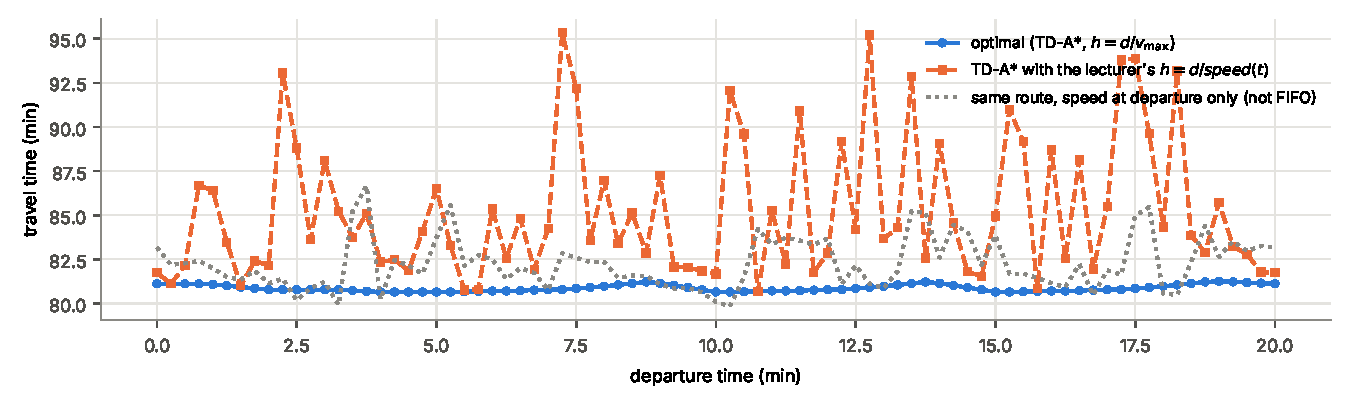
\includegraphics[width=\linewidth]{figures/fig9_td.pdf}
\caption{Part 1: travel time of the longest of the 200 queries as a function
of the departure time (Platform~C).}
\label{fig:td}
\end{figure}

\textbf{The lecturer's heuristic is not admissible, and it shows.} With
$h = d/\mathit{speed}(t)$, 87\% of the 800 runs return a route that is slower
than the optimum, by 4.5\% on average and by up to 29\%. Because the
estimate jumps whenever the clock crosses a slot boundary, the search also
re-opens 45\,665 nodes per query. It is not even faster: it expands more nodes
than the admissible great-circle heuristic (62\,804 against 44\,367).
Figure~\ref{fig:td} shows the same effect for one long trip: the optimal
travel time varies by only 0.6\,min with the departure time, while the
lecturer's heuristic adds up to 14.5\,min. The non-FIFO edge model of the
notebook gives yet another travel time, between 0.9\,min less and 6.0\,min more than the
correct one, because it charges the whole edge at the speed of the slot in which the
car enters it.

\textbf{A better admissible heuristic pays off.} The road distance to the
target divided by $v_{\max}$ is still admissible but much tighter: it needs
43\% fewer expansions than the great-circle heuristic (25\,439 against 44\,367) and is
3.3--3.5$\times$ faster than time-dependent Dijkstra. This is the correct version
of the notebook's \texttt{shortest\_path\_at\_time} idea: compute the road
distances once per destination with a reverse Dijkstra, instead of one full
search per evaluation of $h$.


\subsection{\texorpdfstring{Vector-valued $f$}{Vector-valued f}: multi-objective A*}

With a vector-valued $f$ there is no single optimum. The goal becomes the set
of \textbf{Pareto-optimal} routes, i.e.\ routes that no other route beats in
every objective. We minimise \textbf{(length, congested travel time)}. The two
objectives conflict: short routes use small streets, fast routes use main roads
that are congested at rush hour.

We implement \NAMOA{}~[3]. The scalar $g(v)$ becomes two sets of
non-dominated cost vectors per node, $G_{op}(v)$ and $G_{cl}(v)$. A new label
$(g, v)$ is generated only if no label already stored at $v$ weakly dominates
$g$, and it deletes the labels it dominates. A label is also discarded if its
$f = g + (h_{\mathrm{len}}, h_{\mathrm{time}})$ is weakly dominated by a
solution already found. OPEN is ordered lexicographically by $f$, and the
search stops when OPEN is empty. Every label that reaches the target is a
Pareto-optimal solution, and its parent chain gives the route.

\subsection{Correctness testing}
\label{sec:seq-test}

\texttt{test\_seq} checks six properties. Dijkstra serves as the oracle; it is
simple enough to trust, and the other algorithms must match it exactly.

\begin{itemize}[nosep]
  \item \textbf{T1 Consistency of $h$, exhaustively.} For 5 targets and all 3
        metrics, $h(u) \le w(u,v) + h(v)$ is checked on every one of the
        455\,837 edges.
  \item \textbf{T2 ALT heuristic} (Section~\ref{sec:opt}): consistency on
        every edge, and admissibility against exact distances from a
        reverse Dijkstra.
  \item \textbf{T3 Differential test.} For 300 random pairs and 3 metrics,
        A* (Euclidean and ALT) must return Dijkstra's cost exactly. The path
        must be a real walk from $s$ to $t$ whose edge costs sum to the
        returned cost, and a consistent $h$ must never re-open a node.
  \item \textbf{T4 Bounded sub-optimality.} For
        $\varepsilon\in\{0, 0.1, 0.3, 0.6\}$ and 100 pairs each, both inexact
        heuristics must return a valid path with
        $C^* \le C \le (1+\varepsilon)C^*$, and exactly $C^*$ when
        $\varepsilon=0$.
  \item \textbf{T5 \NAMOA.} For 25 pairs, the front must equal the one found
        by an exhaustive search with $h=0$ point by point. Its points must not
        dominate each other, the cost of each returned path must equal its
        vector, both single-objective optima must be end points of the front,
        and for 16 integer weights $(a,b)$ the best $a\cdot\mathrm{length} +
        b\cdot\mathrm{time}$ on the front must equal an independent Dijkstra
        run on that weighted sum.
  \item \textbf{T6 Time-dependent A*} (Section~\ref{sec:seq-td}): FIFO on
        200\,000 random cases, and agreement with an independent oracle on 100
        queries at random departure times.
\end{itemize}

All six tests pass on all three platforms.

\subsection{Results}

\begin{table}[H]
\centering
\small
\caption{Part 1: exact sequential algorithms, mean over 200 random queries.
Platforms B and C answer the same queries, so their expansion counts are
identical; Platform A uses a different query set (Section~\ref{sec:setup}).}
\label{tab:seq}
\begin{tabular}{ll rr rrrrr}
\toprule
 & & \multicolumn{2}{c}{expanded nodes} & \multicolumn{5}{c}{time per query (ms)} \\
\cmidrule(lr){3-4}\cmidrule(lr){5-9}
Metric & Algorithm & A & B--E & A & B & C & D & E \\
\midrule
length & Dijkstra & 97{,}165 & 104{,}414 & 5.337 & 6.131 & 15.832 & 12.008 & 16.438 \\
 & A*{,} Euclidean $h$ & 22{,}521 & 25{,}806 & 2.159 & 2.656 & 6.366 & 5.337 & 12.683 \\
 & A*{,} ALT 4 landmarks & 11{,}628 & 12{,}096 & 1.428 & 1.504 & 4.109 & 3.417 & 6.746 \\
 & A*{,} ALT 8 landmarks & 7{,}922 & 8{,}696 & 1.161 & 1.271 & 3.751 & 2.833 & 6.072 \\
 & A*{,} ALT 16 landmarks & 6{,}424 & 7{,}026 & 1.365 & 1.349 & 3.727 & 2.945 & 5.906 \\
\midrule
time & Dijkstra & 97{,}818 & 105{,}138 & 6.003 & 6.996 & 19.440 & 13.775 & 18.646 \\
 & A*{,} Euclidean $h$ & 66{,}190 & 71{,}671 & 5.877 & 7.111 & 18.710 & 17.077 & 33.800 \\
\bottomrule
\end{tabular}

\end{table}

\textbf{The heuristic matters more than the hardware.} For length, the
straight-line heuristic cuts expansions $4.0\times$ (104\,414 $\rightarrow$
25\,806) and ALT with 8 landmarks a further $3.0\times$, $12\times$ in total.
Query time follows: 15.8 $\rightarrow$ 3.8\,ms on C and 6.1 $\rightarrow$
1.3\,ms on B. More landmarks still reduce expansions (16 landmarks: 7\,026),
but each evaluation of $h$ then costs more, so ALT-16 is no faster than ALT-8.
For travel time the straight-line bound is weak ($1.5\times$ fewer
expansions), because $v_{\max}$ comes from a few fast trunk-road segments, and
the saved expansions do not pay for computing $h$ (B: 7.1 against 7.0\,ms).
Platform~A answers a query 1.0--1.2$\times$ faster than the Linux VM on the
same chip and about $3\times$ faster than the cloud Xeon (A uses a different
query set; Section~\ref{sec:setup}).

\begin{table}[H]
\centering
\small
\caption{Part 1: uncertain and dynamic heuristics, length metric, 200 queries
on Platform~C. ``mean'' and ``worst'' are cost divided by the optimum;
expanded and re-opened are means per query. The bound is $1+\varepsilon$.}
\label{tab:eps}
\begin{tabular}{r rrrr rrrr}
\toprule
 & \multicolumn{4}{c}{uncertain $h$} & \multicolumn{4}{c}{dynamic $h$} \\
\cmidrule(lr){2-5}\cmidrule(lr){6-9}
$\varepsilon$ & mean & worst & expanded & re-opened & mean & worst & expanded & re-opened \\
\midrule
0.1 & 1.000 & 1.015 & 34{,}909 & 16{,}228 & 1.000 & 1.012 & 43{,}667 & 24{,}031 \\
0.3 & 1.021 & 1.099 & 36{,}539 & 27{,}254 & 1.022 & 1.119 & 32{,}040 & 24{,}310 \\
0.5 & 1.068 & 1.254 & 43{,}302 & 36{,}089 & 1.056 & 1.205 & 40{,}661 & 35{,}920 \\
1.0 & 1.173 & 1.463 & 87{,}936 & 82{,}275 & 1.107 & 1.359 & 76{,}873 & 73{,}801 \\
2.0 & 1.317 & 1.899 & 62{,}745 & 57{,}816 & 1.176 & 1.511 & 51{,}815 & 49{,}450 \\
\bottomrule
\end{tabular}

\end{table}

\begin{figure}[H]
\centering
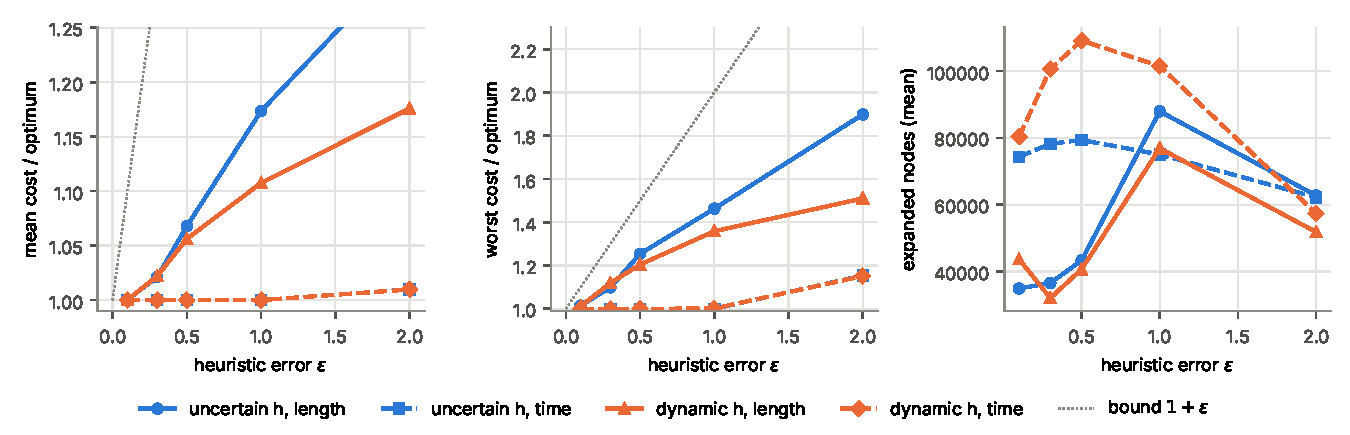
\includegraphics[width=\linewidth]{figures/fig2_eps.pdf}
\caption{Part 1: quality and effort of the inexact heuristics as the error
$\varepsilon$ grows (Platform~C). Dotted line: the guaranteed bound.}
\label{fig:eps}
\end{figure}

\textbf{The loss stays far below the bound.} Up to $\varepsilon=0.3$ the mean
loss is about 2\,\% and the worst case is 9.9\,\% (uncertain) and 11.9\,\%
(dynamic), against a guaranteed 30\,\%. Even at $\varepsilon=2$ the worst
route is 1.90$\times$ the optimum, not 3$\times$. The guarantee is
pessimistic because the error only hurts when the heuristic over-estimates on
the nodes of the optimal path. \textbf{The effort, however, rises sharply.}
Re-openings and stale keys cost so much extra work that the inexact searches
always expand more nodes than A* with the exact straight-line heuristic: 36\,539
(uncertain) and 32\,040 (dynamic) at $\varepsilon=0.3$, and 87\,937 at
$\varepsilon=1$, against 25\,806. The dynamic heuristic needs far more lazy
re-keying than the uncertain one (81\,446 against 13\,064 stale pops per query
at $\varepsilon=0.3$), because its error drifts in one direction for hundreds
of expansions. For travel time the loss is smaller still: the time heuristic
is so weak that even a doubled estimate rarely over-estimates (worst case 1.15
at $\varepsilon=2$).

\begin{figure}[H]
\centering
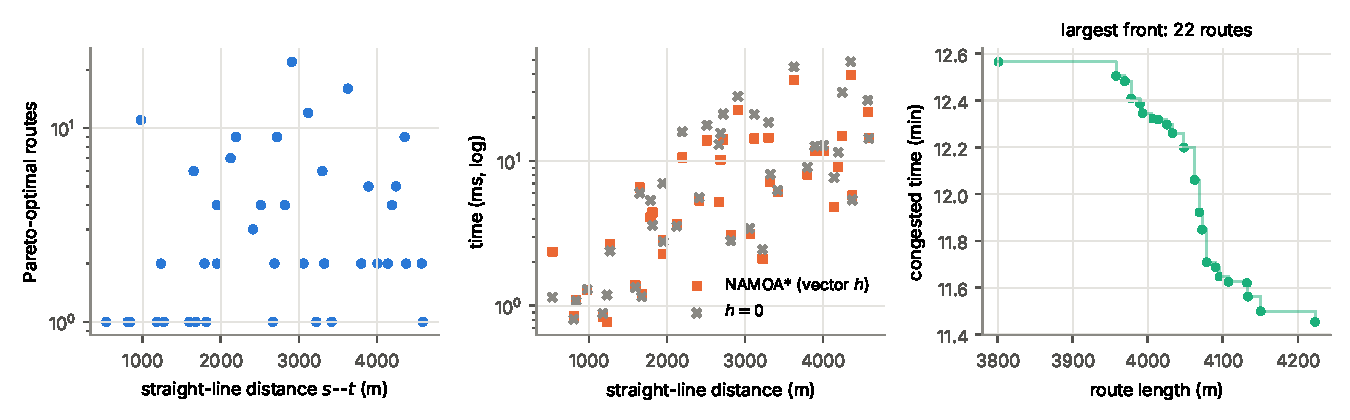
\includegraphics[width=\linewidth]{figures/fig3_namoa.pdf}
\caption{Part 1: \NAMOA{} on 40 queries of increasing distance (Platform~C):
size of the Pareto front (left), run time against the uninformed search with
$h=0$ (middle), and the largest front found (right).}
\label{fig:namoa}
\end{figure}

\textbf{Vector-valued $f$.} The number of Pareto-optimal routes ranges from 1
to 22 (median 2) and depends on the shape of the city between $s$ and $t$ more
than on the distance. When main roads and side streets run parallel, many
trade-offs exist; otherwise one route is best in both objectives. The front
size decides the cost: on Platform~C the query with 22 routes takes 22.6\,ms,
while queries with a single Pareto-optimal route take 0.8--14\,ms. The vector
heuristic makes \NAMOA{} expand $1.7\times$ fewer labels (median) than the
same search with $h=0$, and the exhaustive cross-checks of T5 found no
difference between the two fronts.

\paragraph{Dynamic world: re-planning while driving.} To use A* in a world
that changes, we simulated 40 trips of at least 3.5\,km on the travel-time
metric. Every 15 driven edges, three traffic jams (3--8$\times$ slower, radius
300\,m) appear on the road ahead. Strategy~1 keeps following the initial plan.
Strategy~2 re-plans with A* from the current position after each update; a
jam only increases costs, so the straight-line $h$ stays admissible.

\begin{figure}[H]
\centering
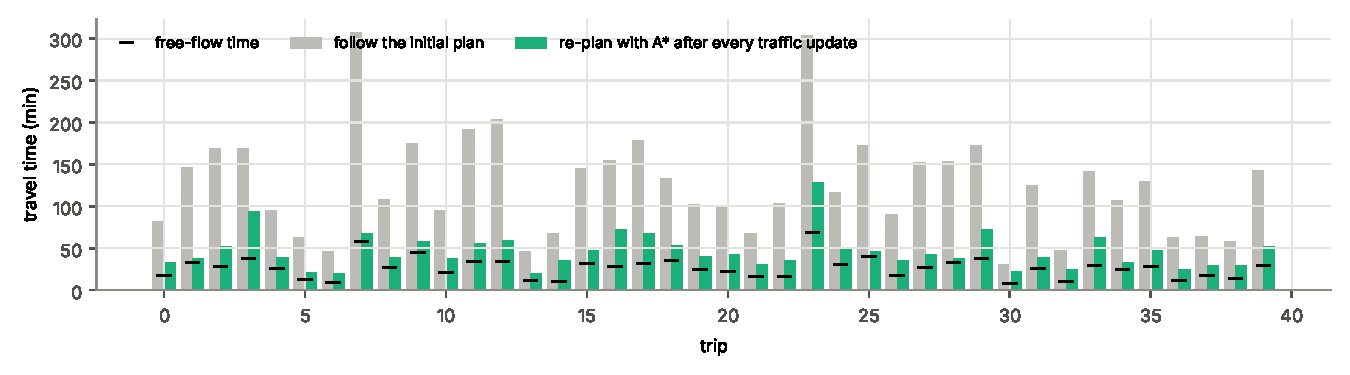
\includegraphics[width=\linewidth]{figures/fig4_dynamic.pdf}
\caption{Part 1: travel time of 40 simulated trips when traffic jams appear
while driving (Platform~C).}
\label{fig:dynamic}
\end{figure}

Re-planning reduces the mean trip from 125.5 to 45.9 minutes (free-flow time
26.6 minutes) and is never worse than following the initial plan. It needs on
average 16.5 re-plans per trip of 16.5\,ms each on Platform~C (6.0\,ms on B),
which is fast enough to run on every traffic update.

% Section: clist (\input from main.tex)
\section{The Concurrent Set Data Structure}
\label{sec:clist}

\subsection{Implementation}

The set is a sorted singly linked list with two sentinel nodes, \texttt{head}
(key $-\infty$) and \texttt{tail} (key $+\infty$), and offers \texttt{add},
\texttt{remove} and \texttt{contains}~[1]. The assignment asks
for two of the four synchronization strategies; we implemented all four,
because Part~3 compares all of them as an open list. Each list is a template
over its lock type. Each list also has a \texttt{removeMin} operation, which
Part~3 needs to use the set as a priority queue.

\paragraph{Coarse-grained.} One lock protects the whole list. Every operation
is a sequential traversal inside one critical section.

\paragraph{Fine-grained.} Every node has its own lock and a traversal uses
\emph{hand-over-hand} locking: a thread locks the next node before releasing
the current one, so it always holds two adjacent locks. Threads can work on
different parts of the list at once, but they can never overtake each other.

\paragraph{Optimistic.} A thread first searches without any locks, then locks
the two nodes \texttt{pred} and \texttt{curr} it found, and finally
\emph{validates} them by traversing from \texttt{head} again to check that
\texttt{pred} is still reachable and still points to \texttt{curr}. If not, it
releases the locks and retries.

\paragraph{Lazy.} Each node has a \texttt{marked} flag. Removal first sets the
flag (logical deletion) and then unlinks the node (physical deletion).
Validation becomes a constant-time local check, and \texttt{contains} takes no
locks at all and is wait-free:

\begin{lstlisting}
bool remove(Key k) {
  for (Backoff b;; b.backoff()) {
    Node* pred = head; Node* curr = pred->next.load(std::memory_order_acquire);
    while (curr->key < k) { pred = curr; curr = curr->next.load(std::memory_order_acquire); }
    pred->lock(); curr->lock();
    if (!pred->marked && !curr->marked && pred->next == curr) {   // validate
      bool ok = curr->key == k;
      if (ok) {
        curr->marked.store(true, std::memory_order_release);           // logical
        pred->next.store(curr->next.load(), std::memory_order_release); // physical
      }
      curr->unlock(); pred->unlock();
      if (ok) retire(curr);
      return ok;
    }
    curr->unlock(); pred->unlock();                                  // retry
  }
}
bool contains(Key k) {                                               // wait-free
  Node* curr = head;
  while (curr->key < k) curr = curr->next.load(std::memory_order_acquire);
  return curr->key == k && !curr->marked.load(std::memory_order_acquire);
}
\end{lstlisting}

\paragraph{Locks.} We used three locks: \texttt{std::mutex}; a TTAS spinlock;
and a TTAS lock with \textbf{exponential backoff}, as in Assignment~1. After
seeing the lock busy, or losing the race for it, a thread waits a random number
of \texttt{pause}/\texttt{yield} instructions in $[0, \textit{limit})$ and
doubles \textit{limit} up to 1\,024; at the cap it also calls
\texttt{std::this\_thread::yield()}. The optimistic and lazy lists also back
off after a failed validation.

\paragraph{Memory ordering and reclamation.} \texttt{next} pointers and
\texttt{marked} flags are \texttt{std::atomic}. Stores that publish a node use
\texttt{release} and traversals use \texttt{acquire}, so a thread that reaches
a node through a pointer also sees the node's key and successor. The lock-free
traversals are therefore free of data races under the C++ memory model,
including on ARM. A node unlinked by one thread may still be visited by a
concurrent optimistic or lazy traversal, so it cannot be freed at once. Removed
nodes are pushed onto a lock-free \emph{retired} stack and freed when the list
is destroyed. A long-running service would need hazard pointers or epoch-based
reclamation instead.

\paragraph{\texttt{removeMin}.} The minimum is always the first node after
\texttt{head}. Every variant locks \texttt{head} and that node (or, in the
coarse list, the whole list), validates the pair as above, and unlinks the node.

\subsection{Correctness testing}

\texttt{test\_clist} runs every one of the 12 list/lock combinations with 1, 2,
4 and 8 threads:

\begin{itemize}[nosep]
  \item \textbf{(a) Sequential specification.} 20\,000 random operations,
        \texttt{removeMin} included, are compared with \texttt{std::set}.
  \item \textbf{(b) Disjoint keys.} Each thread inserts and then removes its own
        residue class of keys. The size, the order and finally the emptiness
        of the list are checked.
  \item \textbf{(c) Overlapping keys.} Threads run random
        \texttt{add}/\texttt{remove}/\texttt{contains} on 64 shared keys and
        count their \emph{successful} adds and removes per key. If the set is
        linearizable, then for each key the initial membership plus all
        successful adds minus all successful removes must be 0 or 1 and equal
        its final membership. One lost update breaks this. Concurrently,
        keys that are never removed must always be found and keys that are
        never inserted must never be found.
  \item \textbf{(d) Concurrent \texttt{removeMin}.} All threads drain 6\,000
        keys. Every key must come out exactly once, and the keys each thread
        receives must be strictly increasing.
  \item \textbf{(e) Producers and consumers} exchange keys through
        \texttt{add}/\texttt{removeMin}; nothing may be lost or duplicated.
  \item \textbf{ThreadSanitizer.} The same tests built with
        \texttt{-fsanitize=thread} report no data race.
\end{itemize}

All tests pass on all five platforms. Testing also exposed a performance
problem: with plain TTAS locks and 8 threads on the 2 cores of Platform~C, the
fine-grained list needed 97\,s for the test suite, against 1.6\,s with the
backoff lock. A preempted thread holding a node lock blocks the whole
hand-over-hand chain behind it, and the waiting threads burn their time slices
spinning.

\subsection{Results}

\textbf{Usage scenario.} The set is an ordered in-memory index shared by the
worker threads of a routing service, with keys in $[0, 1000)$ and the list
pre-filled to half. Three workload mixes are measured:
\emph{read} (90\% \texttt{contains}, 5\% \texttt{add}, 5\% \texttt{remove}),
\emph{update} (50/25/25), and \emph{priority queue} (50\% \texttt{add}, 50\%
\texttt{removeMin}), which is how Part~3 uses the list.

\begin{figure}[H]
\centering
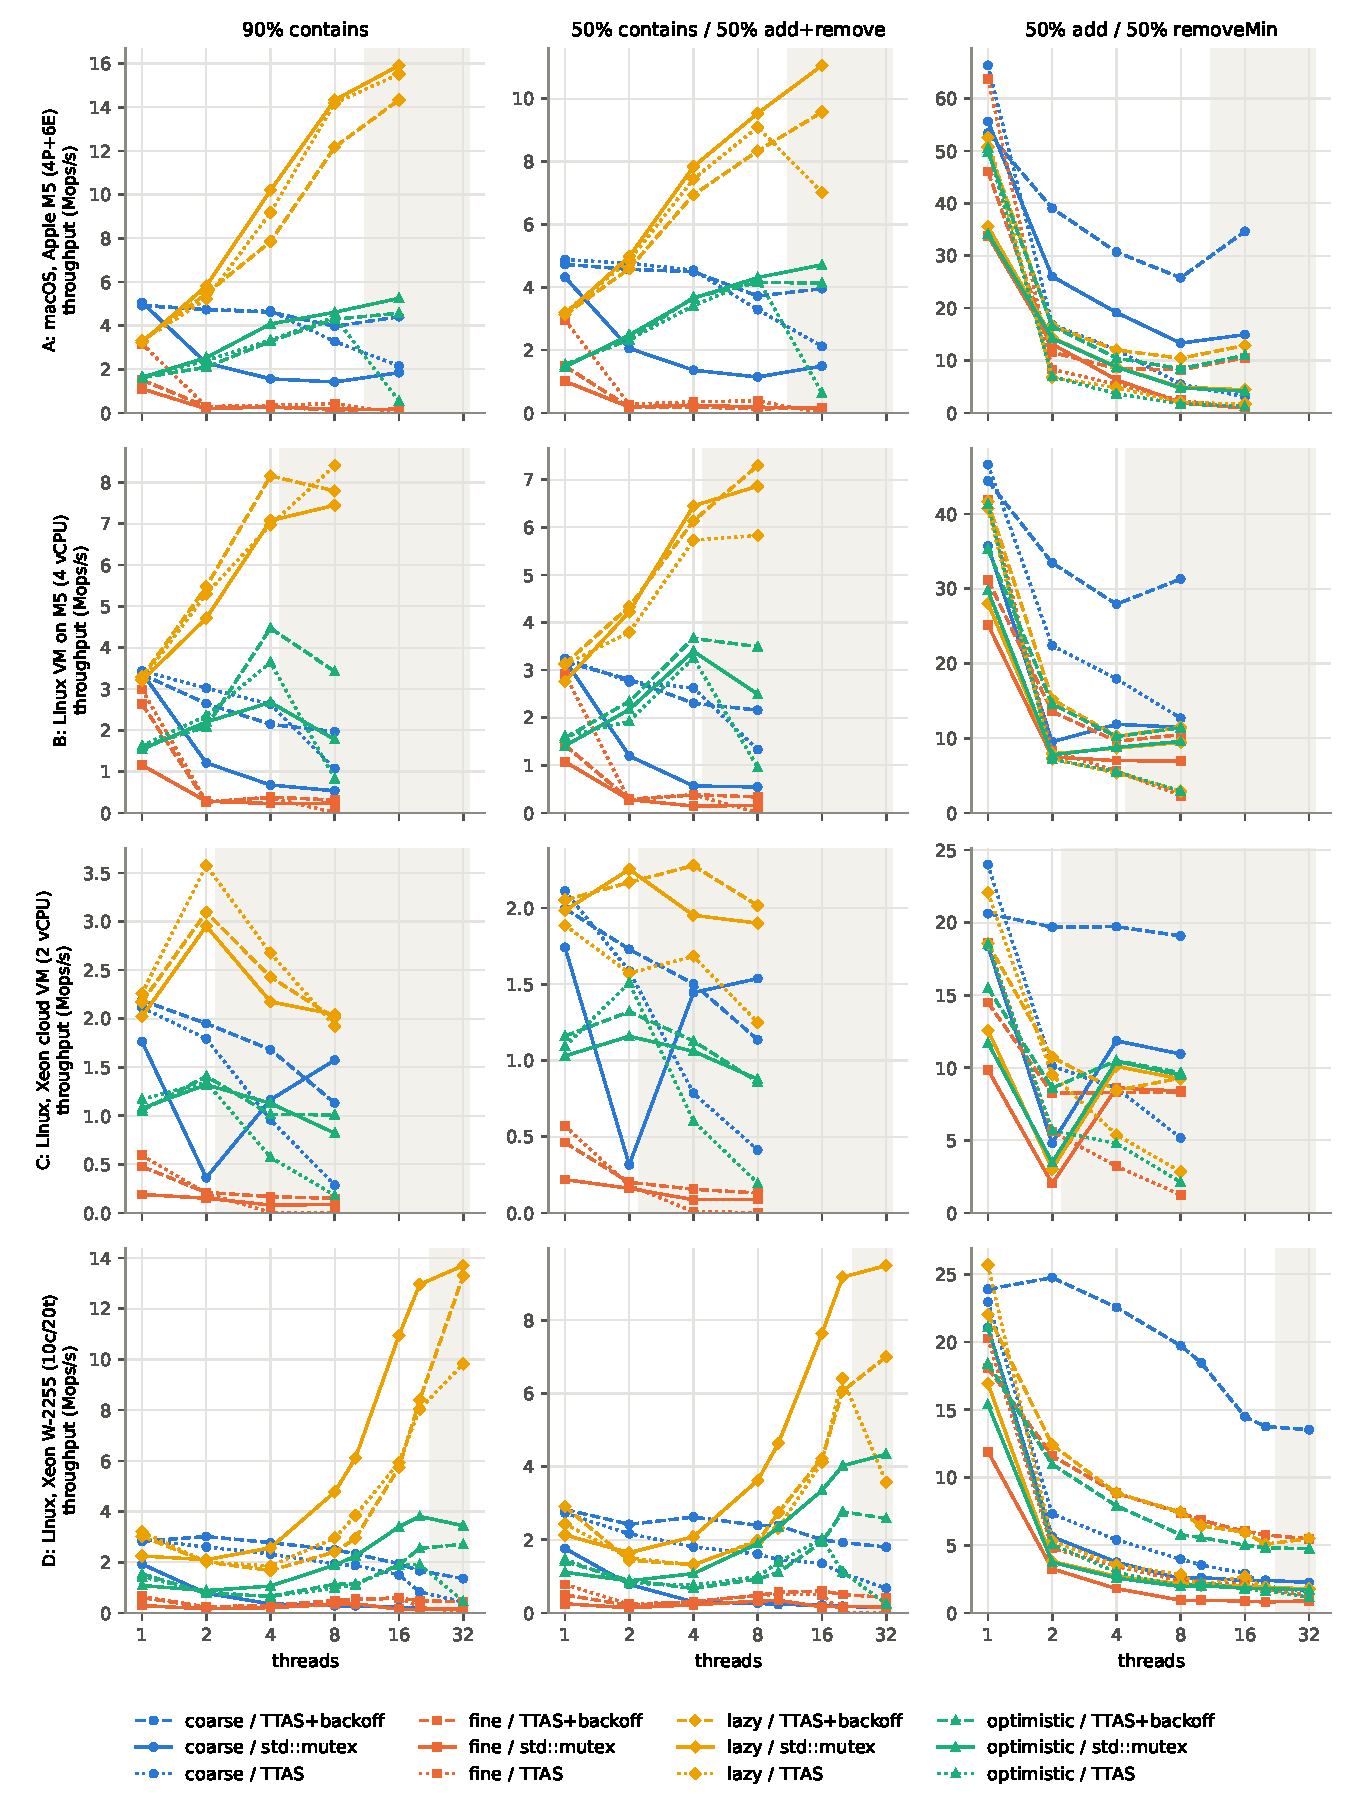
\includegraphics[width=\linewidth]{figures/fig5_clist.pdf}
\caption{Part 2: throughput of the 12 list/lock combinations on the four
platforms (rows) for the three workload mixes (columns). Median of 3 runs of
0.4\,s. Colour: list; line style: lock. The shaded region marks
oversubscription.}
\label{fig:clist}
\end{figure}

\begin{table}[H]
\centering
\scriptsize
\setlength{\tabcolsep}{4pt}
\caption{Part 2: throughput (million operations/s) for the read mix and the
priority-queue mix. TTAS rows are omitted (see Figure~\ref{fig:clist}).}
\label{tab:clist}
\begin{tabular}{lrrrrrrrrrrrr}
\toprule
 & \multicolumn{6}{c}{90\% \texttt{contains} (threads)} & \multicolumn{6}{c}{\texttt{add}/\texttt{removeMin} (threads)} \\
\cmidrule(lr){2-7}\cmidrule(lr){8-13}
List / lock & 1 & 2 & 4 & 8 & 16 & 32 & 1 & 2 & 4 & 8 & 16 & 32 \\
\midrule
\multicolumn{13}{l}{\emph{Platform A (macOS, Apple M5)}} \\
Coarse, \texttt{std::mutex} & 5.1 & 2.3 & 1.6 & 1.4 & 1.8 & -- & 55.6 & 26.0 & 19.2 & 13.3 & 14.9 & -- \\
Coarse, TTAS+backoff & 4.9 & 4.7 & 4.6 & 4.0 & 4.4 & -- & 53.4 & 39.1 & 30.7 & 25.8 & 34.7 & -- \\
Fine-grained, \texttt{std::mutex} & 1.1 & 0.2 & 0.3 & 0.2 & 0.2 & -- & 33.8 & 13.1 & 6.3 & 2.0 & 0.9 & -- \\
Fine-grained, TTAS+backoff & 1.5 & 0.3 & 0.3 & 0.1 & 0.2 & -- & 46.1 & 11.6 & 8.5 & 8.2 & 10.5 & -- \\
Optimistic, \texttt{std::mutex} & 1.6 & 2.5 & 4.1 & 4.6 & 5.2 & -- & 34.2 & 14.2 & 8.7 & 4.8 & 4.1 & -- \\
Optimistic, TTAS+backoff & 1.6 & 2.1 & 3.3 & 4.3 & 4.6 & -- & 49.8 & 16.6 & 10.5 & 8.4 & 11.0 & -- \\
Lazy, \texttt{std::mutex} & 3.2 & 5.8 & 10.2 & 14.3 & 15.9 & -- & 35.5 & 14.4 & 8.8 & 4.9 & 4.4 & -- \\
Lazy, TTAS+backoff & 3.3 & 5.5 & 7.8 & 12.2 & 14.3 & -- & 50.8 & 16.6 & 12.0 & 10.4 & 12.9 & -- \\
\midrule
\multicolumn{13}{l}{\emph{Platform B (Linux VM, 4 vCPU)}} \\
Coarse, \texttt{std::mutex} & 3.4 & 1.2 & 0.7 & 0.5 & -- & -- & 35.7 & 9.5 & 11.9 & 11.5 & -- & -- \\
Coarse, TTAS+backoff & 3.4 & 2.6 & 2.1 & 2.0 & -- & -- & 44.4 & 33.5 & 27.9 & 31.3 & -- & -- \\
Fine-grained, \texttt{std::mutex} & 1.2 & 0.3 & 0.2 & 0.2 & -- & -- & 25.2 & 7.5 & 7.0 & 6.9 & -- & -- \\
Fine-grained, TTAS+backoff & 2.6 & 0.3 & 0.4 & 0.3 & -- & -- & 31.1 & 13.6 & 9.6 & 10.5 & -- & -- \\
Optimistic, \texttt{std::mutex} & 1.5 & 2.2 & 2.7 & 1.8 & -- & -- & 29.8 & 7.8 & 8.8 & 9.6 & -- & -- \\
Optimistic, TTAS+backoff & 1.6 & 2.1 & 4.5 & 3.4 & -- & -- & 35.3 & 14.6 & 10.2 & 11.4 & -- & -- \\
Lazy, \texttt{std::mutex} & 3.2 & 4.7 & 7.1 & 7.4 & -- & -- & 28.0 & 7.9 & 8.7 & 9.4 & -- & -- \\
Lazy, TTAS+backoff & 3.3 & 5.5 & 8.2 & 7.8 & -- & -- & 41.7 & 15.2 & 10.3 & 11.5 & -- & -- \\
\midrule
\multicolumn{13}{l}{\emph{Platform C (Linux, Xeon, 2 vCPU)}} \\
Coarse, \texttt{std::mutex} & 1.8 & 0.4 & 1.2 & 1.6 & -- & -- & 18.4 & 4.8 & 11.9 & 11.0 & -- & -- \\
Coarse, TTAS+backoff & 2.2 & 1.9 & 1.7 & 1.1 & -- & -- & 20.6 & 19.7 & 19.7 & 19.1 & -- & -- \\
Fine-grained, \texttt{std::mutex} & 0.2 & 0.2 & 0.1 & 0.1 & -- & -- & 9.9 & 2.0 & 8.6 & 8.4 & -- & -- \\
Fine-grained, TTAS+backoff & 0.5 & 0.2 & 0.2 & 0.1 & -- & -- & 14.5 & 8.3 & 8.3 & 8.3 & -- & -- \\
Optimistic, \texttt{std::mutex} & 1.1 & 1.3 & 1.1 & 0.8 & -- & -- & 11.7 & 3.5 & 10.5 & 9.5 & -- & -- \\
Optimistic, TTAS+backoff & 1.1 & 1.4 & 1.0 & 1.0 & -- & -- & 15.5 & 8.6 & 10.5 & 9.7 & -- & -- \\
Lazy, \texttt{std::mutex} & 2.0 & 3.0 & 2.2 & 2.0 & -- & -- & 12.6 & 3.0 & 10.1 & 9.2 & -- & -- \\
Lazy, TTAS+backoff & 2.2 & 3.1 & 2.4 & 2.0 & -- & -- & 18.6 & 10.7 & 8.4 & 9.3 & -- & -- \\
\midrule
\multicolumn{13}{l}{\emph{Platform D (Linux, Xeon W-2255, 10c/20t)}} \\
Coarse, \texttt{std::mutex} & 1.9 & 0.8 & 0.4 & 0.3 & 0.2 & 0.1 & 21.1 & 5.6 & 3.7 & 2.5 & 2.4 & 2.3 \\
Coarse, TTAS+backoff & 2.8 & 3.0 & 2.8 & 2.5 & 1.9 & 1.4 & 23.9 & 24.8 & 22.6 & 19.7 & 14.5 & 13.5 \\
Fine-grained, \texttt{std::mutex} & 0.3 & 0.2 & 0.2 & 0.3 & 0.1 & 0.2 & 11.9 & 3.3 & 1.8 & 0.9 & 0.9 & 0.9 \\
Fine-grained, TTAS+backoff & 0.6 & 0.2 & 0.3 & 0.5 & 0.6 & 0.4 & 18.1 & 11.6 & 8.8 & 7.4 & 6.0 & 5.5 \\
Optimistic, \texttt{std::mutex} & 1.1 & 0.9 & 1.1 & 1.9 & 3.4 & 3.4 & 15.4 & 3.7 & 2.6 & 1.9 & 1.8 & 1.7 \\
Optimistic, TTAS+backoff & 1.5 & 0.8 & 0.7 & 1.1 & 1.9 & 2.7 & 18.4 & 11.0 & 7.9 & 5.8 & 5.0 & 4.7 \\
Lazy, \texttt{std::mutex} & 2.2 & 2.1 & 2.6 & 4.8 & 10.9 & 13.7 & 16.9 & 3.8 & 2.7 & 2.2 & 2.0 & 1.8 \\
Lazy, TTAS+backoff & 3.0 & 2.0 & 1.7 & 2.4 & 5.7 & 13.3 & 22.0 & 12.4 & 8.8 & 7.4 & 6.0 & 5.5 \\
\midrule
\multicolumn{13}{l}{\emph{Platform E (Windows, i5-9300H, 4c/8t)}} \\
Coarse, \texttt{std::mutex} & 2.5 & 1.1 & 0.9 & 0.8 & -- & -- & 11.4 & 6.6 & 4.6 & 5.1 & -- & -- \\
Coarse, TTAS+backoff & 2.0 & 1.9 & 1.7 & 1.4 & -- & -- & 8.4 & 8.3 & 6.4 & 5.0 & -- & -- \\
Fine-grained, \texttt{std::mutex} & 0.1 & 0.2 & 0.2 & 0.1 & -- & -- & 5.6 & 2.6 & 2.2 & 2.2 & -- & -- \\
Fine-grained, TTAS+backoff & 0.1 & 0.1 & 0.1 & 0.1 & -- & -- & 3.9 & 3.9 & 3.3 & 2.8 & -- & -- \\
Optimistic, \texttt{std::mutex} & 1.0 & 1.2 & 2.1 & 2.9 & -- & -- & 4.6 & 2.5 & 1.6 & 0.9 & -- & -- \\
Optimistic, TTAS+backoff & 1.0 & 1.0 & 1.1 & 1.6 & -- & -- & 3.7 & 3.0 & 2.5 & 2.0 & -- & -- \\
Lazy, \texttt{std::mutex} & 2.3 & 2.6 & 3.8 & 5.6 & -- & -- & 4.1 & 2.5 & 1.5 & 0.9 & -- & -- \\
Lazy, TTAS+backoff & 2.3 & 3.0 & 2.9 & 4.6 & -- & -- & 4.3 & 3.5 & 3.3 & 2.4 & -- & -- \\
\bottomrule
\end{tabular}

\end{table}

Figure~\ref{fig:clist} and Table~\ref{tab:clist} summarize the sweep.

\textbf{Only the lazy list scales.} With the read mix, the lazy list goes from
3.2 to 15.9\,Mops/s on Platform~A ($5\times$ at 16 threads), from 3.3 to
8.2\,Mops/s on Platform~B ($2.5\times$ at 4 threads), and to 13.7\,Mops/s on Platform~D (32 threads; 9.5\,Mops/s on \emph{update}). Its \texttt{contains}
takes no lock, and \texttt{add}/\texttt{remove} lock only two neighbouring
nodes after a lock-free search. The optimistic list scales less (1.6
$\rightarrow$ 4.6\,Mops/s on A) because its validation traverses the list a
second time. The coarse list cannot scale: with backoff it stays flat
(4.9 $\rightarrow$ 4.4\,Mops/s on A), and with \texttt{std::mutex} it degrades.

\textbf{The fine-grained list is the slowest.} A traversal of about 250 nodes
acquires and releases about 250 locks, and because threads cannot overtake
each other, the slowest thread sets the pace for all. Already at 2 threads it
falls to 0.3\,Mops/s or less on every platform (read mix).

\textbf{\texttt{removeMin} does not scale on any list.} In the priority-queue
mix every \texttt{removeMin} needs the same two nodes at the head of the list,
so the list behaves like one lock. Throughput drops as soon as a second thread
arrives (on A, 66 $\rightarrow$ 17\,Mops/s with TTAS on the coarse list) and
the variant with the cheapest critical section wins: the coarse list with
backoff, which loses least (53 $\rightarrow$ 26\,Mops/s at 8 threads on A,
and nearly flat at about 20\,Mops/s on C). This is the bottleneck that Part~3
inherits.

\textbf{Locks.} \texttt{std::mutex} collapses as soon as two threads contend on
Linux (coarse list, priority-queue mix on B: 35.7 $\rightarrow$
9.5\,Mops/s), because each contended hand-off puts a thread to sleep in the
kernel and wakes it up again. Pure TTAS collapses under oversubscription
(fine-grained list on A: 3.2 $\rightarrow$ 0.0\,Mops/s at 16 threads),
because waiting threads spin while the lock holder is descheduled. TTAS with
backoff is the best or nearly the best lock in almost every configuration. One
exception is the lazy list on macOS, where \texttt{std::mutex} is as good as
backoff (15.9 against 14.3\,Mops/s): the lazy list's locks are rarely
contended, and Apple's mutex spins briefly before it sleeps.

% Section: parallel (\input from main.tex)
\section{A* in the Parallel World}
\label{sec:par}

\subsection{Why the two parts do not merge directly}

Using the sorted list of Section~\ref{sec:clist} as the OPEN list of the A* of
Section~\ref{sec:seq} fails for four reasons:

\begin{enumerate}[nosep]
  \item The list is a \emph{set} of distinct keys, but OPEN holds $(f, v)$
        pairs and many nodes share the same $f$.
  \item The list has no operation that removes the minimum.
  \item The CLOSED set and the $g$ and parent arrays would be read and written
        by several threads without synchronization.
  \item The two stopping rules of sequential A* become wrong. The first goal
        popped is not necessarily optimal, because another thread may still be
        expanding a cheaper node. An empty OPEN does not mean the search is
        over, because another thread may be about to insert children.
\end{enumerate}

\subsection{Adaptations}\label{sec:par-adapt}

\paragraph{The list.} The key becomes the 64-bit integer $(f \ll 24) \mid v$.
Keys are unique per node and $f$ value, and their order is the order of $f$.
Inserting the same node twice with the same $f$ is a harmless duplicate that
\texttt{add} rejects. \texttt{removeMin} was added to every list
(Section~\ref{sec:clist}).

\paragraph{The search.} There is no CLOSED set. The $g$-value and the parent of
each node are packed into one 64-bit \texttt{std::atomic} and lowered with a
compare-and-swap loop, so $g$ and parent always belong together. Whenever
$g(v)$ improves, $v$ is inserted again. A node can therefore be expanded more
than once; these extra expansions are the \emph{search overhead} of parallel
A*. A popped entry with $f > g(u) + h(u)$ is stale and skipped. An
\emph{incumbent} $U$ holds the cost of the best path to the goal found so far
(an atomic minimum). Entries with $f \ge U$ are neither inserted nor expanded.

\paragraph{Termination.} A counter \texttt{pending} holds the number of
outstanding work items: the entries in OPEN plus the entries that a thread has
popped and is still processing. It starts at 1 (the source). Before a thread
inserts the children of a node it reserves one item per outgoing edge; when all
children are in OPEN it releases the reservations it did not use together with
the popped entry itself. \texttt{pending} therefore never under-counts, and it
can reach zero only when OPEN is empty and no thread holds an entry, after
which no thread can create work any more. A thread that finds OPEN empty stops
the search exactly when \texttt{pending} is zero. Two separate reads (``OPEN is
empty'', then ``no thread is busy'') would not be enough: between the two reads
another thread can insert its children and finish, and the search would stop
with work left in OPEN. \texttt{push} reports whether the entry was really
added, because the list is a set and rejects a duplicate key.

\begin{lstlisting}
std::atomic<long> pending{1};                            // the source
while (!done.load(std::memory_order_acquire)) {
  Key k;
  if (!open.pop(k)) {                                    // removeMin
    if (pending.load() == 0) { done = true; break; }
    backoff(); continue;
  }
  Cost f = key_f(k); int u = key_v(k);
  Cost gu = unpack_g(G[u].load(std::memory_order_acquire));
  if (f > gu + h(u) || f >= U.load()) { pending.fetch_sub(1); continue; } // stale / pruned
  if (u == t) { atomic_min(U, gu); pending.fetch_sub(1); continue; }
  long reserved = graph.degree(u), added = 0;
  pending.fetch_add(reserved);                           // before any child is inserted
  for (auto e = graph.begin(u); e != graph.end(u); ++e) {
    Cost ng = gu + e->w;
    if (cas_min_g(G[e->to], ng, u)) {                    // g and parent in one CAS
      if (e->to == t) atomic_min(U, ng);
      if (ng + h(e->to) < U.load() && open.push(make_key(ng + h(e->to), e->to))) added++;
    }
  }
  pending.fetch_sub(reserved - added + 1);               // unused reservations + this entry
}
\end{lstlisting}

\paragraph{Why the result is optimal.} When the search stops, \texttt{pending} is
zero: OPEN is empty and no thread is expanding, so every node whose $g$ was ever lowered to a value
with $f < U$ has been expanded with its final $g$. Take an optimal path
$s = v_0, \dots, v_k = t$ and suppose some node on it ends with
$g(v_i) > g^*(v_i)$; take the first one. Its predecessor ended with the optimal
$g^*(v_{i-1})$ and, because $h$ is consistent, with
$f \le C^* \le U$, so it was expanded and lowered $g(v_i)$ to $g^*(v_i)$ ---
a contradiction. Hence $g(t) = C^*$. The parent chain is a real path of that
cost: if a parent's final $g$ plus the edge cost were smaller than its child's
$g$, the parent would have been expanded again and would have improved the
child.

\subsection{Versions compared}

\begin{center}
\small
\begin{tabularx}{\linewidth}{>{\raggedright\arraybackslash}p{3.6cm} >{\raggedright\arraybackslash}p{3.3cm} Y}
\toprule
\textbf{Version} & \textbf{OPEN list} & \textbf{Notes} \\
\midrule
sequential A*   & binary heap & Section~\ref{sec:seq}; baseline for all speed-ups \\
list: coarse / fine / optimistic / lazy & shared sorted list & the adapted lists of Part~2, each with \texttt{std::mutex} and with TTAS+backoff (8 versions) \\
shared heap     & binary heap + one lock & $O(\log n)$ operations, but one lock serializes everything \\
\HDA            & one private heap per thread & Hash-Distributed A*~[5]: node $v$ belongs to thread $\mathrm{hash}(v) \bmod T$; generated nodes are sent in batches to the owner's mailbox; termination through a global count of outstanding work \\
\HDA{} + $f$-window & as \HDA & a thread waits while its best $f$ is more than 3\% above the smallest $f$ published by any thread (Section~\ref{sec:opt}) \\
\bottomrule
\end{tabularx}
\end{center}

\subsection{Correctness testing}

\texttt{test\_par} picks 30 random $(s, t)$ pairs on the city graph (one with
$s = t$) and runs 11 version/heuristic combinations with 1, 2, 4 and 8
threads: 1\,320 runs per platform and 3\,960 in total. Every run must return
\emph{exactly} the Dijkstra-optimal cost, and its path must start at $s$, end
at $t$, use only existing edges and have an edge sum equal to the returned
cost. The different thread counts and repeated runs exercise many
interleavings, and 8 threads on 2 or 4 cores force threads to be preempted
inside critical sections. The suite was also run under ThreadSanitizer.

All 3\,960 runs pass and ThreadSanitizer reports no data race. In the
benchmarks below, the mean and the worst cost/optimum ratio are 1.000000 for
every version, so the versions differ only in time.

\subsection{Results}

Each benchmark answers 20 long queries (straight-line distance $> 5$\,km;
about 100\,000 Dijkstra expansions each). We measured four heuristics:
$h = 0$ (parallel Dijkstra), Euclidean, ALT with 8 landmarks, and a
\emph{costly} heuristic. The costly heuristic returns the Euclidean value but
performs 400 dependent floating-point operations per evaluation (about
0.5--1\,$\mu$s). It stands for an expensive predictor, such as a learned
travel-time model, and lets us vary the amount of work per expansion. With
$h = 0$ the list versions were left out: with OPEN lists of thousands of
entries they would take hours.

\begin{figure}[H]
\centering
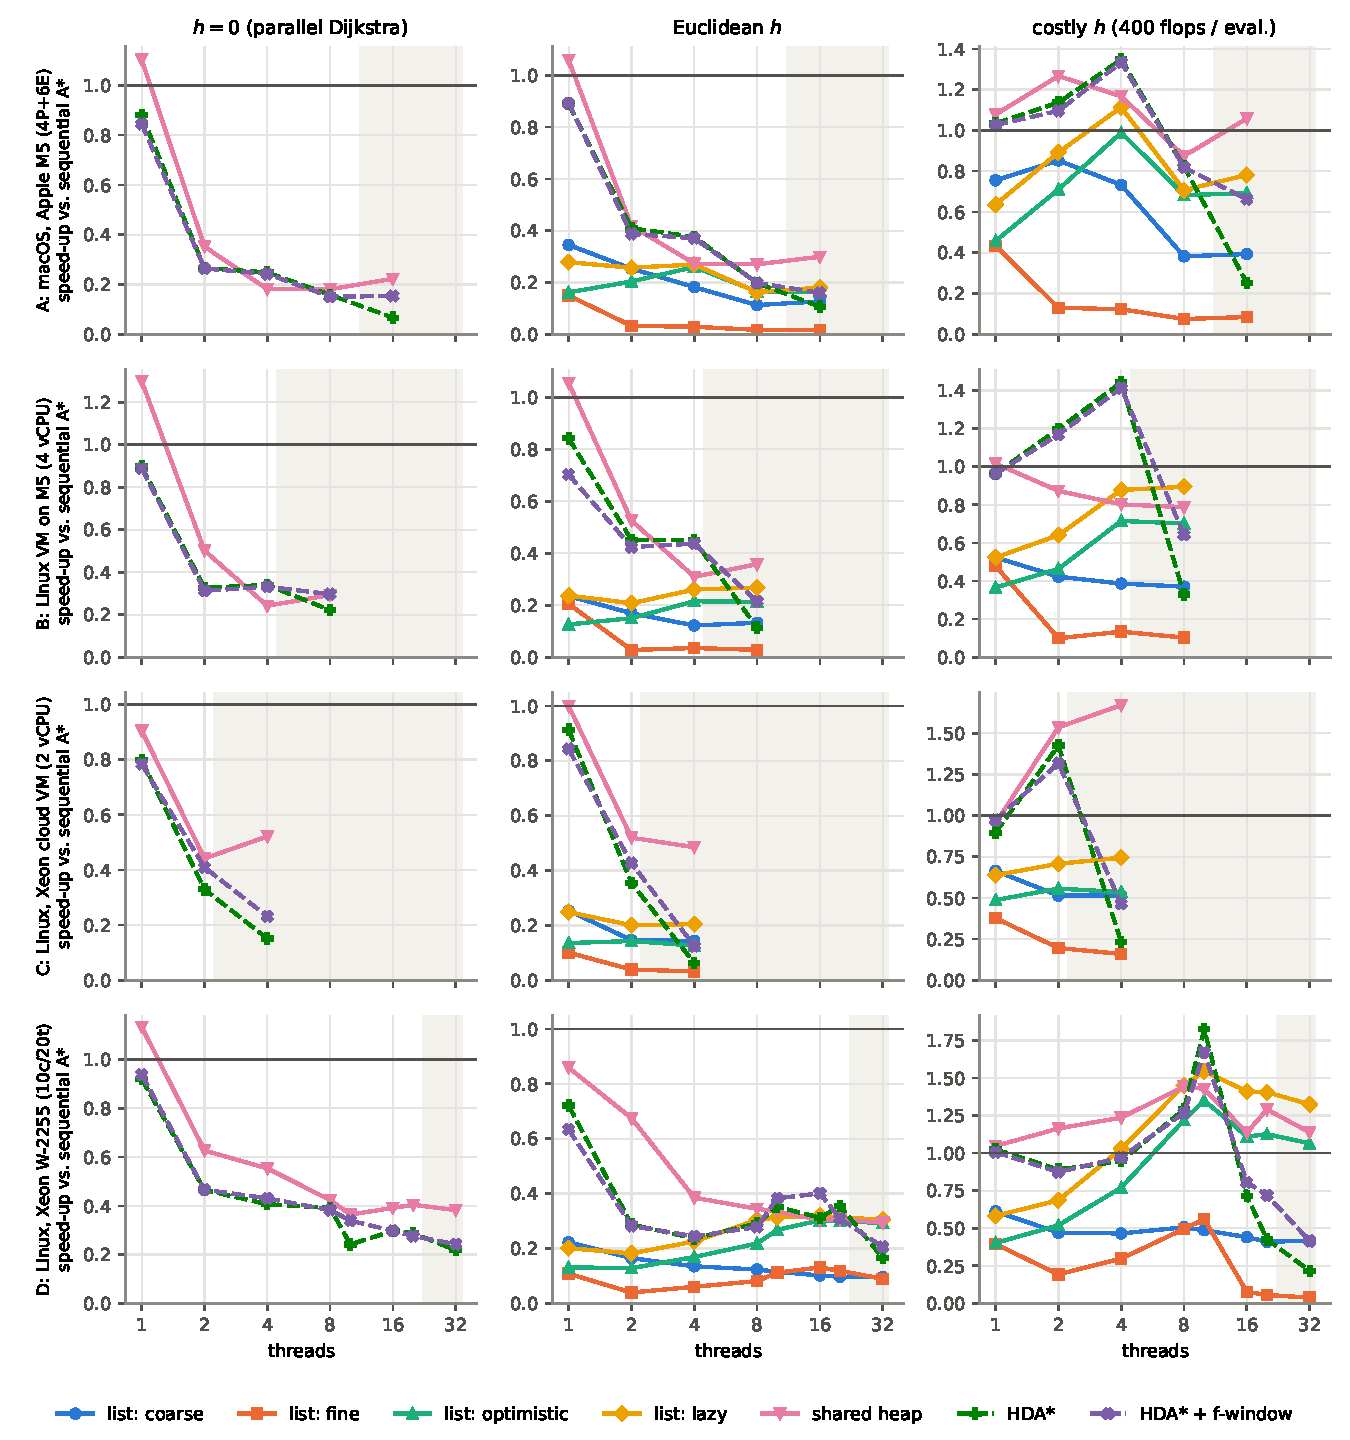
\includegraphics[width=\linewidth]{figures/fig6_astar.pdf}
\caption{Part 3: speed-up of parallel A* over sequential A* on the three
platforms (rows) for three heuristics (columns); 20 long queries, median of 3
runs. Solid lines: shared OPEN list (lists and heap with TTAS+backoff); dashed:
\HDA. The shaded region marks oversubscription.}
\label{fig:astar}
\end{figure}

\begin{table}[H]
\centering
\scriptsize
\setlength{\tabcolsep}{4pt}
\caption{Part 3: wall time (ms) to answer 20 long queries. Bold: faster than
sequential A* on the same platform. Locks are TTAS+backoff unless stated.}
\label{tab:astar}
\begin{tabular}{lrrrrrrrrrr}
\toprule
 & \multicolumn{5}{c}{Euclidean $h$ (threads)} & \multicolumn{5}{c}{costly $h$ (threads)} \\
\cmidrule(lr){2-6}\cmidrule(lr){7-11}
Version & 1 & 2 & 4 & 8 & 16 & 1 & 2 & 4 & 8 & 16 \\
\midrule
\multicolumn{11}{l}{\emph{Platform A (macOS, Apple M5)}} \\
sequential A* & 40 &  &  &  &  & 169 &  &  &  &  \\
list: coarse & 115 & 157 & 218 & 353 & 312 & 224 & 198 & 231 & 442 & 429 \\
list: fine & 265 & 1229 & 1379 & 2374 & 2674 & 390 & 1303 & 1376 & 2267 & 2002 \\
list: optimistic & 246 & 195 & 153 & 241 & 241 & 369 & 238 & 171 & 247 & 244 \\
list: lazy & 143 & 154 & 147 & 243 & 221 & 266 & 189 & \textbf{152} & 239 & 216 \\
list: lazy, \texttt{std::mutex} & 156 & 276 & 273 & 442 & 428 & 279 & 298 & 285 & 475 & 451 \\
shared heap & \textbf{37} & 95 & 145 & 147 & 132 & \textbf{157} & \textbf{133} & \textbf{145} & 193 & \textbf{160} \\
shared heap, \texttt{std::mutex} & \textbf{40} & 96 & 151 & 228 & 210 & \textbf{158} & 246 & 251 & 409 & 346 \\
HDA* & 45 & 97 & 105 & 200 & 373 & \textbf{163} & \textbf{149} & \textbf{125} & 205 & 670 \\
HDA* + $f$-window & 44 & 102 & 107 & 200 & 248 & \textbf{164} & \textbf{154} & \textbf{127} & 206 & 255 \\
\midrule
\multicolumn{11}{l}{\emph{Platform B (Linux VM, 4 vCPU)}} \\
sequential A* & 39 &  &  &  &  & 143 &  &  &  &  \\
list: coarse & 166 & 231 & 319 & 294 & -- & 273 & 338 & 370 & 386 & -- \\
list: fine & 190 & 1394 & 1101 & 1370 & -- & 298 & 1433 & 1065 & 1385 & -- \\
list: optimistic & 309 & 259 & 181 & 183 & -- & 390 & 308 & 200 & 203 & -- \\
list: lazy & 164 & 188 & 150 & 145 & -- & 273 & 223 & 163 & 160 & -- \\
list: lazy, \texttt{std::mutex} & 194 & 191 & 179 & 179 & -- & 287 & 235 & 195 & 191 & -- \\
shared heap & \textbf{37} & 74 & 126 & 109 & -- & \textbf{141} & 164 & 178 & 181 & -- \\
shared heap, \texttt{std::mutex} & \textbf{38} & 127 & 137 & 154 & -- & \textbf{143} & 270 & 252 & 258 & -- \\
HDA* & 46 & 86 & 87 & 343 & -- & 148 & \textbf{119} & \textbf{99} & 434 & -- \\
HDA* + $f$-window & 55 & 92 & 89 & 181 & -- & 148 & \textbf{122} & \textbf{101} & 222 & -- \\
\midrule
\multicolumn{11}{l}{\emph{Platform C (Linux, Xeon, 2 vCPU)}} \\
sequential A* & 91 &  &  &  &  & 464 &  &  &  &  \\
list: coarse & 360 & 624 & 636 & -- & -- & 699 & 902 & 900 & -- & -- \\
list: fine & 907 & 2329 & 2831 & -- & -- & 1232 & 2368 & 2904 & -- & -- \\
list: optimistic & 673 & 638 & 723 & -- & -- & 953 & 834 & 867 & -- & -- \\
list: lazy & 367 & 456 & 446 & -- & -- & 727 & 656 & 624 & -- & -- \\
list: lazy, \texttt{std::mutex} & 455 & 490 & 581 & -- & -- & 848 & 686 & 703 & -- & -- \\
shared heap & 91 & 176 & 188 & -- & -- & 486 & \textbf{302} & \textbf{278} & -- & -- \\
shared heap, \texttt{std::mutex} & \textbf{91} & 455 & 157 & -- & -- & 501 & 549 & \textbf{400} & -- & -- \\
HDA* & 100 & 257 & 1449 & -- & -- & 518 & \textbf{326} & 1996 & -- & -- \\
HDA* + $f$-window & 108 & 214 & 730 & -- & -- & 477 & \textbf{352} & 999 & -- & -- \\
\bottomrule
\end{tabular}

\end{table}

\textbf{With a cheap heuristic, no parallel version is faster.} With the
Euclidean or ALT heuristic, or with $h = 0$, one expansion takes about
0.2--0.4\,$\mu$s: three or four edges and a few array accesses. That is about
the cost of one operation on the shared OPEN list, plus the cache misses on
its head. Adding threads therefore adds synchronization and cache-coherence
traffic faster than it adds useful work. From 2 threads on, every version
runs at 0.79$\times$ the speed of sequential A* or slower, on every platform
(Figure~\ref{fig:astar}, left and middle columns).

\textbf{A sorted list is a poor priority queue on a large graph.} Even with
one thread the list versions are 3--14$\times$ slower than the binary heap
with the Euclidean heuristic. Insertion walks the list, so it costs
$O(|\textrm{OPEN}|)$ instead of $O(\log |\textrm{OPEN}|)$, and on the city
graph OPEN holds thousands of nodes. The gap shrinks as the heuristic gets
better (ALT: 1.4--4$\times$), because a better heuristic keeps OPEN smaller.
With more threads every \texttt{removeMin} also competes for the head of the
list, which is exactly the priority-queue bottleneck measured in Part~2. The
ranking of the lists is the same as in Part~2: lazy (and optimistic) with
backoff are the best, fine-grained is by far the worst.

\textbf{Parallelism pays off only when expansions are expensive.} With the
costly heuristic (right column), several versions beat sequential A*: \HDA{}
reaches $1.35\times$ on Platform~A and $1.44\times$ on B (both at 4 threads),
and the shared heap with backoff reaches $1.27\times$ on A and $1.67\times$ on
C. On a large graph the lists also profit from more threads, because several
threads can walk the long list at the same time: on Platform~A the lazy list
goes from $0.64\times$ with one thread to $1.11\times$ with 4, the first
list-based parallel A* that is faster than sequential A*, and the optimistic
list from $0.46\times$ to $0.99\times$. On Platform~A every version slows down
again beyond 4 threads, although the machine has 10 cores: only 4 of them are
performance cores, and in a search that all threads share, the slowest thread
holds the others back. \texttt{std::mutex} is never the better lock here (lazy
list on A: $0.59\times$ against $1.11\times$ with backoff at 4 threads),
because the critical sections last only a few hundred nanoseconds, much less
than a sleep and wake-up in the kernel.

\begin{figure}[H]
\centering
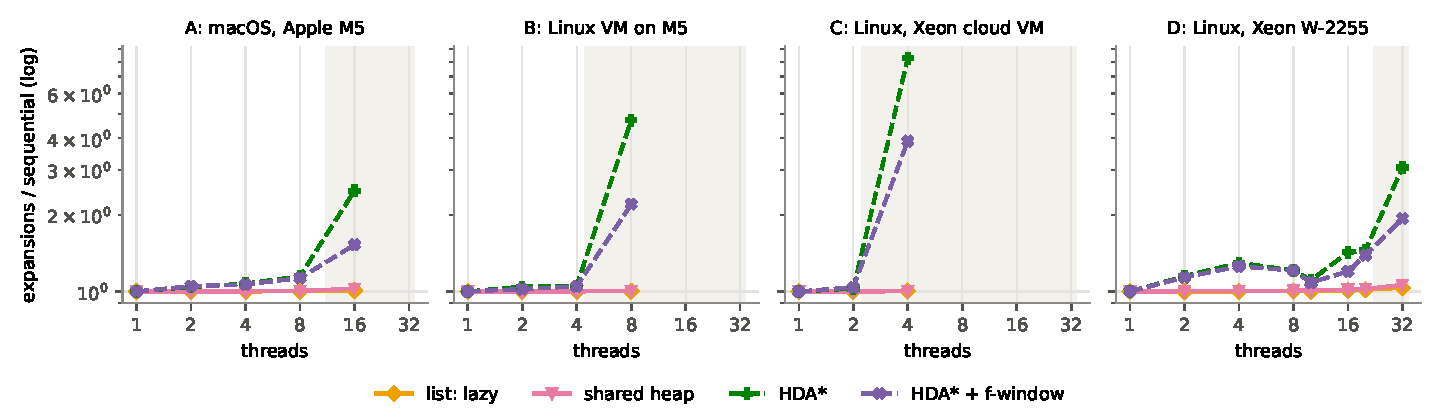
\includegraphics[width=\linewidth]{figures/fig7_overhead.pdf}
\caption{Part 3: search overhead with the Euclidean heuristic: expanded nodes
divided by those of sequential A*. Shaded: oversubscription.}
\label{fig:overhead}
\end{figure}

\textbf{\HDA{} trades contention for search overhead.} \HDA{} has no shared
OPEN list, so it does not suffer the bottleneck at the head. It also has no
global $f$-order, and Figure~\ref{fig:overhead} shows the price. While every
thread has its own core it expands at most 15\% more nodes than sequential A*
with the Euclidean heuristic. When a thread is descheduled, the nodes it owns
stop moving, the path to the goal stalls, and the other threads keep expanding
nodes far beyond the optimal $f$ because $U$ is still infinite: on Platform~C
\HDA{} expands $8\times$ more nodes than sequential A* at 4 threads ($21\times$
with ALT). The shared OPEN list stays within 20\% at every thread count,
because its threads always take the globally best node.

% Section: optimizations (\input from main.tex)
\section{Other Optimizations (optional)}
\label{sec:opt}

The lecture lists four directions for Assignment~2: priority queues with
different synchronization schemes (Part~3), contraction hierarchies, pruning
and labeling. This section covers the last three.

\paragraph{ALT landmarks (labeling).} ALT (A*, Landmarks, Triangle
inequality)~[4] improves the heuristic with precomputed
distances. We pick $k$ landmarks by farthest-point selection and store the
distances from and to every landmark $L$, computed with one forward and one
reverse Dijkstra per landmark. The triangle inequality then gives
\[
  h(v) = \max\Bigl(h_{\mathrm{euclid}}(v),\;
         \max_L \bigl(d(L,t) - d(L,v)\bigr),\;
         \max_L \bigl(d(v,L) - d(t,L)\bigr)\Bigr),
\]
which is admissible and consistent (test T2 checks this on every edge). Each
node thus carries a label of $2k$ distances. For $k=8$ the preprocessing takes
0.2--0.7\,s and 26\,MB. Expansions fall from 25\,806 (Euclidean) to 12\,096,
8\,696 and 7\,026 for $k = 4, 8, 16$, and query time by $1.7$--$2.1\times$
(Table~\ref{tab:seq}); beyond 8 landmarks the cost of evaluating $h$ eats the
savings. ALT also works in every parallel version, but it makes each search
so short that no parallel version gets above $0.79\times$ the sequential speed
with 2 or more threads.

\paragraph{Pruning with an incumbent.} In all parallel versions, entries with
$f \ge U$ are neither inserted nor expanded. In \HDA{}, a thread whose best
local $f$ reaches $U$ discards its whole heap at once.

\paragraph{Heuristic memoisation.} For a static heuristic, $h(v)$ is computed
at most once per query and cached in an array of relaxed atomics that all
threads share. Without the cache, a node's $h$ is evaluated again in the stale check of
every pop. This matters for the costly heuristic, and the cache makes every
version, sequential or parallel, pay for each $h(v)$ exactly once, so their
times are comparable.

\paragraph{$f$-window for \HDA.} Each \HDA{} thread publishes the $f$ of its best
local node. A thread expands its node only if
$f \le (1 + 0.03)\cdot \min_{\text{threads}} f$; otherwise it yields. This
keeps all threads close to the global $f$-frontier and does not affect
optimality, since it only delays expansions. It reduces the search overhead of
\HDA{} under oversubscription from $8.3\times$ to $3.9\times$ at 4 threads on
Platform~C, from $4.7\times$ to $2.2\times$ at 8 threads on B, and from
$2.5\times$ to $1.5\times$ at 16 threads on A (Euclidean heuristic,
Figure~\ref{fig:overhead}).

\paragraph{Smaller items.} \HDA{} sends generated nodes in batches (one lock
per destination per expansion), and threads that find no work back off
exponentially and yield the CPU to threads that hold work.

\paragraph{Contraction hierarchies.} We did not implement them. Preprocessing
the 203\,k-node city graph would take seconds, but each query would shrink to
a few hundred expansions, which leaves even less work to divide among threads. For a routing
service, answering \emph{different} queries in parallel is then the better use
of the cores.

% Section: cross_platform (\input from main.tex)
\section{Cross-Platform Comparison}
\label{sec:cross}

The three platforms differ in core count (10, 4 and 2), in core types (A mixes
performance and efficiency cores), in instruction set and memory model (ARMv8
on A and B, x86-64 on C), and in operating system and C++ library (macOS with
libc++ on A, Linux with libstdc++ on B and C). Platforms A and B run on the
same Apple M5 chip, natively and inside a virtual machine.
Table~\ref{tab:cross} summarizes the best result of each part on each platform,
and Figure~\ref{fig:cross} compares how the key results scale.

\begin{table}[H]
\centering
\small
\caption{Best result per platform. ``$\times$'' values are speed-ups over
sequential A* on the same platform; thread counts in parentheses.}
\label{tab:cross}
\begin{tabularx}{\linewidth}{l YYY}
\toprule
 & \textbf{A: macOS, M5, 10 cores} & \textbf{B: Linux VM, 4 vCPU} & \textbf{C: Linux, Xeon, 2 vCPU} \\
\midrule
Sequential A*, Euclidean $h$ (city graph) & 2.2\,ms / query & 2.7\,ms / query & 6.4\,ms / query \\
Best list, 90\% \texttt{contains} & lazy, \texttt{std::mutex}: 15.9\,Mops/s (16) & lazy, TTAS: 8.4\,Mops/s (8) & lazy, TTAS: 3.6\,Mops/s (2) \\
Best list, \texttt{add}/\texttt{removeMin}, $\ge 2$ threads & coarse, backoff: 39.1\,Mops/s (2) & coarse, backoff: 33.5\,Mops/s (2) & coarse, backoff: 19.7\,Mops/s (2) \\
Best parallel A*, Euclidean $h$ & $0.42\times$ (shared heap, 2) & $0.53\times$ (shared heap, 2) & $0.58\times$ (shared heap, \texttt{std::mutex}, 4) \\
Best parallel A*, costly $h$ & $1.35\times$ (\HDA, 4) & $1.44\times$ (\HDA, 4) & $1.67\times$ (shared heap, 4) \\
Best list-based parallel A*, costly $h$ & $1.11\times$ (lazy, 4) & $0.89\times$ (lazy, 8) & $0.74\times$ (lazy, 4) \\
\bottomrule
\end{tabularx}
\end{table}

\begin{figure}[H]
\centering
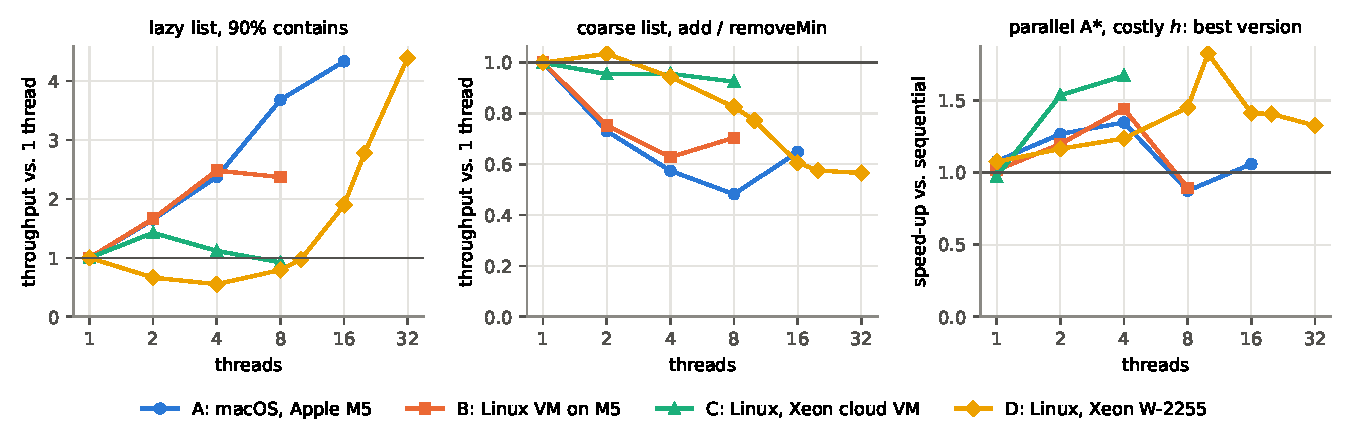
\includegraphics[width=\linewidth]{figures/fig8_cross.pdf}
\caption{Cross-platform scaling: lazy list with the read mix (left), coarse
list with \texttt{add}/\texttt{removeMin} (middle), and the best parallel A*
version at each thread count with the costly heuristic (right).}
\label{fig:cross}
\end{figure}

\textbf{Core count decides how far the lazy list scales.} The lazy list is the
best concurrent set on every platform, and its read throughput keeps growing
for as long as there are cores: up to 16 threads on A ($4.3\times$ with backoff, $5\times$ with \texttt{std::mutex}), 4 on B
($2.5\times$) and 2 on C ($1.4\times$). Its traversals never write shared
memory, so readers do not slow each other down. After the last core, the
curves flatten (A) or fall (B, C).

\textbf{A priority queue at the head does not scale anywhere.}
\texttt{add}/\texttt{removeMin} loses throughput as soon as a second thread
arrives, on every platform and for every list (Figure~\ref{fig:cross},
middle). Many cores do not help when every operation needs the same two
nodes. This is the main reason why parallel A* over a shared OPEN list is
slower than sequential A* on all three machines unless expansions are costly.

\textbf{The granularity of the work matters more than the platform.} With a
cheap heuristic, the best parallel A* is slower than sequential A* on every
platform, and a 10-core laptop does no better than a 2-vCPU cloud machine.
Only with the costly heuristic does parallel A* win on all three platforms
(1.35--1.67$\times$). The best version differs per platform: \HDA, which has no
shared queue, wins on the two ARM platforms; the shared heap wins on the x86 VM.

\textbf{A larger graph helps the lists.} On the city graph OPEN is long, and
several threads can walk it at the same time. The lazy list therefore gains
from extra threads on every platform with the costly heuristic, and on
Platform~A it becomes the first list-based parallel A* that beats sequential
A* ($1.11\times$ at 4 threads). It still loses clearly to the heap at one
thread, because its operations are linear in the size of OPEN.

\textbf{Heterogeneous cores limit Platform~A.} Platform~A has the most cores but
gives the smallest best speed-up for parallel A* (1.35$\times$), and the Linux
VM on the same chip does better with the same 4 threads (1.44$\times$). A search
that all threads share advances at the pace of its slowest thread. From 5
threads on, some threads must run on efficiency cores; macOS may also place
some of the first 4 threads there, whereas the VM's 4 virtual CPUs are
scheduled by the hypervisor. Throughput-oriented code such as the lazy list,
where threads do not wait for each other, uses all 10 cores well.

\textbf{Oversubscription hurts spinning most.} On Platform~C, 4 threads run on 2
virtual CPUs and 8 threads in Part~2. Pure TTAS spinlocks collapse there, and so
does plain \HDA{} ($8\times$ search overhead at 4 threads). Locks and loops that
back off and yield, and the $f$-window for \HDA, keep the damage small. One
result on C we cannot fully explain: the shared heap with the costly heuristic
is fastest at 4 threads on 2 vCPUs ($1.67\times$, against $1.54\times$ at 2
threads), on the city graph as on the small graph. A possible reason is that
the hypervisor gives the VM more physical capacity than 2 vCPUs suggest; we did
not verify this.

\textbf{Memory model.} The same code passed every correctness test on the weak
ARMv8 memory model (A, B) and on x86-64 TSO (C), and ThreadSanitizer found no
data race. Because every shared access uses \texttt{std::atomic} with explicit
acquire/release ordering, no platform-specific code was needed.

% Section: limitations (\input from main.tex)
\section{Limitations and Threats to Validity}
\label{sec:threats}

\begin{itemize}
  \item \textbf{Platforms A and B share one chip, and B and C are VMs.} Platforms A and
        B both run on the same Apple M5, and Platforms B and C are virtual
        machines whose virtual CPUs are scheduled by a hypervisor we do not
        control. Bare-metal Platform~D (Intel Xeon W-2255, 10 cores / 20 threads)
        removes hypervisor noise, though it ran on a shared workstation with light
        background activity ($\text{load average} \approx 3.5$).
  \item \textbf{Different query sets.} \texttt{std::\allowbreak uniform\_int\_\allowbreak distribution}
        differs between libc++ and libstdc++, so Platform~A answered other
        random queries than B and C. Speed-ups are computed per platform and
        remain comparable, but absolute times and expansion counts of A should
        not be compared with B and C directly.
  \item \textbf{Short runs.} A Part~3 configuration (20 queries) takes
        19\,ms to 4.3\,s, so a single query often lasts only a few
        milliseconds. At this scale, OS noise and CPU
        frequency changes are visible. We report medians of 3 repetitions
        only, without spread.
  \item \textbf{Part~3 on Platforms~A and~C predates the final termination
        rule.} An earlier version of the shared-OPEN search stopped when OPEN
        was empty and a counter of busy threads was zero, read one after the
        other. That left a rare race, which we never observed in normal runs
        and could only trigger with injected delays; the \texttt{pending}
        counter of Section~\ref{sec:par-adapt} removes it. Platform~B was
        measured again with the final code: the times of the affected versions
        changed by about 3\,\% (median), as much as those of the versions whose
        code did not change, and every cost stayed optimal. The Part~3 times
        and test runs of Platforms~A and~C in this report were taken with the
        earlier version. The final code also passes \texttt{test\_par} on an
        x86-64 Linux VM of the same kind as Platform~C.
  \item \textbf{Thread start-up and short-run spread.} In the standard sweep, every
        parallel query creates and joins its $T$ threads and reports medians of 3
        repetitions without spread. The extended Platform~D suite (\texttt{run\_ext.sh})
        isolates search scaling via a persistent \texttt{ThreadPool}, pins threads to
        physical cores first, and reports 7-repetition standard deviation, IQR, and
        per-query $p_{95}$/$p_{99}$ latencies.
  \item \textbf{Graph built without OSMnx.} Because Nominatim was blocked
        and Overpass overloaded, the city graph comes from Geofabrik's extract
        with our own filter and simplification, cut by a bounding box rather
        than by the administrative boundary. It keeps service roads (except
        parking aisles and driveways), which OSMnx's \texttt{drive} network
        partly drops, so node counts differ from the lecturer's notebook.
  \item \textbf{Unequal sweeps.} Part~3 used up to $2\times$ the hardware
        threads, i.e.\ only $\{1,2,4\}$ on Platform~C, and left out the list
        versions with $h = 0$ because they would run for hours.
  \item \textbf{Synthetic parts of the workload.} The costly heuristic adds
        artificial work to model an expensive predictor, the dynamic and
        uncertain heuristics are noise models, and the congestion factors and
        traffic jams are invented, and the lecturer's speed profile is the same on
        every road. The road graph itself is real.
  \item \textbf{Memory is reclaimed late.} Removed list nodes are freed only
        when the list is destroyed. This is safe and fine for one search, but
        a long-running server would need hazard pointers or epoch-based
        reclamation.
  \item \textbf{No tuning sweep.} The backoff limits (1\,024 for locks, 256
        for validation retries) and the 3\% $f$-window were chosen once and not
        tuned per platform.
  \item \textbf{No thread pinning.} Threads were not pinned to cores, so on
        Platform~A we cannot tell how many of them ran on efficiency cores.
\end{itemize}

% Section: conclusion (\input from main.tex)
\section*{Conclusion}
\addcontentsline{toc}{section}{Conclusion}

We implemented sequential A* on a 203\,396-node road graph of urban Ho Chi
Minh City built from OpenStreetMap, extended it to uncertain and dynamic
heuristics, to the lecturer's time-dependent speed model and to a
vector-valued $f$ (\NAMOA), implemented the four sorted-list concurrent sets
with three locks each, and combined both into parallel A*, alongside a locked
heap and \HDA. We also checked the lecture's pseudocode and reference notebook,
found ten problems in the notebook (the most serious makes every road segment
cost 1\,m) and provide a corrected, tested version. Every exact algorithm was
checked against an independent oracle for exact cost equality on thousands of
random queries, and the concurrent code also under ThreadSanitizer; all tests
pass on all four platforms. The study supports five conclusions:

\begin{enumerate}[nosep]
  \item \textbf{A better heuristic beats more threads.} ALT landmarks make a
        query $12\times$ smaller than Dijkstra; no parallel version of a
        single query came close to that gain.
  \item \textbf{Inexact heuristics cost effort, not much quality.} Uncertain
        and dynamic heuristics lose far less than their bound $1+\varepsilon$,
        but the re-openings they cause make the search slower. The lecturer's
        $h = d/\mathit{speed}(t)$ is not admissible and returns a slower route
        in most runs (87--91\%); dividing by the maximum speed fixes this.
  \item \textbf{The lazy list is the concurrent set that scales.} Its wait-free
        \texttt{contains} reaches $5\times$ on 10 cores. Fine-grained locking
        is the slowest design, and spinning without backoff collapses
        whenever threads outnumber cores.
  \item \textbf{A sorted list is a poor open list.} \texttt{removeMin} always
        contends at the head and insertion is linear. A list-based parallel A*
        is correct after four adaptations, but only the lazy list with an
        expensive heuristic beat sequential A* ($1.11\times$ on 4 performance cores on A; $1.55\times$ on 10 uniform Xeon cores on D).
  \item \textbf{Parallel A* needs coarse work per node.} On a road graph a node
        expansion takes less than a microsecond, and with a cheap heuristic
        every parallel version loses to sequential A*. With an expensive
        heuristic, \HDA{} and the shared heap reach $1.35$--$1.83\times$ ($1.91\times$ with a persistent pool and core pinning on D). For
        many short queries, running different queries in parallel is the
        better use of the cores.
\end{enumerate}

% Section: references (\input from main.tex)
\section*{References}
\addcontentsline{toc}{section}{References}
{\raggedright
\begin{enumerate}[label={[\arabic*]},nosep,leftmargin=*]
  \item \label{ref:herlihy} M.~Herlihy, N.~Shavit, V.~Luchangco, M.~Spear.
        \emph{The Art of Multiprocessor Programming}, 2nd ed. Morgan Kaufmann,
        2020 (Ch.~7 Spin locks and contention; Ch.~9 Linked lists: the role of
        locking).
  \item P.~E.~Hart, N.~J.~Nilsson, B.~Raphael. A formal basis for the
        heuristic determination of minimum cost paths. \emph{IEEE Trans.\
        Systems Science and Cybernetics} 4(2):100--107, 1968.
  \item \label{ref:mandow} L.~Mandow, J.~L.~P\'erez de la Cruz.
        Multiobjective A* search with consistent heuristics. \emph{Journal of
        the ACM} 57(5), 2010.
  \item \label{ref:goldberg} A.~V.~Goldberg, C.~Harrelson. Computing the
        shortest path: A* search meets graph theory. \emph{SODA}, 2005.
  \item \label{ref:kishimoto} A.~Kishimoto, A.~Fukunaga, A.~Botea.
        Evaluation of a simple, scalable, parallel best-first search strategy.
        \emph{Artificial Intelligence} 195:222--248, 2013.
  \item OpenStreetMap contributors. Map data of Ho Chi Minh City, Open
        Database License (ODbL), \url{https://www.openstreetmap.org}.
  \item ISO/IEC 14882:2017, Programming languages --- C++
        (\texttt{std::atomic}, \texttt{std::thread}).
\end{enumerate}
}


\appendix
% Section: appendix (\input from main.tex)
\section{Reproducing the Results}

\begin{lstlisting}[language=bash]
make                       # build all programs into bin/
make test                  # correctness tests (Parts 1-3) on the small graph
make tsan                  # the concurrent tests under ThreadSanitizer
./run_all.sh <platform>    # Part 2 and the small graph -> results/
./run_city.sh <platform>   # Parts 1 and 3 on the city graph -> results_city/
bash run_mac.sh; bash run_mac_city.sh      # macOS: the same two steps
# optional: rebuild data_city/ from Geofabrik's extract
python3 scripts/pbf_to_graph.py vietnam-latest.osm.pbf data_city
# figures, tables and PDF
cd report/latex
python3 scripts/make_figures.py ../../results_city ../../results ../../data_city figures
python3 scripts/make_tables.py ../../results_city ../../results tables
latexmk -pdf main.tex
# the lecturer's example query
./bin/route 10.768856 106.725019 10.839613 106.845798 --algo alt --data data_city
\end{lstlisting}

\section{Work Distribution}

\begin{center}
\begin{tabularx}{\linewidth}{l X}
\toprule
\textbf{Member} & \textbf{Contribution} \\
\midrule
Pham Hoang Son & \todo{contribution} \\
Nguyen Hoang Nam & \todo{contribution} \\
Nguyen Dinh Khanh & \todo{contribution}; Platforms~A and B (Apple M5) runs \\
\bottomrule
\end{tabularx}
\end{center}


\end{document}
